\documentclass[12pt,a4paper]{article}

%Packages
% \usepackage{textcomp}
% \usepackage{latexsym}
% \usepackage{url}
% \usepackage{epsfig}
% \usepackage{graphicx}
% \usepackage{amssymb}
% \usepackage{amsmath}
% \usepackage{mathtools}
% \usepackage{bm}
% \usepackage{array}
% \usepackage[version=3]{mhchem}
% \usepackage{ifthen}
% \usepackage{caption}
% \usepackage{amsthm}
% \usepackage{amstext}
% \usepackage{enumerate}
% \usepackage[osf]{mathpazo}
% \usepackage{dcolumn}

\usepackage[margin=2cm]{geometry}
\usepackage{lscape}
\usepackage{hyperref}
\usepackage{lineno}
\usepackage{pdflscape}
\usepackage{mathtools}
\usepackage[osf]{mathpazo}
\usepackage{fullpage}
\usepackage{float}
\usepackage{ltablex}
\usepackage{longtable}
\usepackage[tablewithin=none,figurewithin=none,singlelinecheck=false]{caption}

\pagenumbering{arabic}

\renewcommand{\thefigure}{S\arabic{figure}} 
 \renewcommand{\thetable}{S\arabic{table}}

%-------------------------------------------------------------------------------
% Title page information
%-------------------------------------------------------------------------------

\title{Supplementary Materials from: \textit{Innovation and elaboration on the avian tree of life}; Science Advances, in review}

\author{Thomas Guillerme, 
Jen A. Bright,
Christopher R. Cooney\\
Emma C. Hughes,
Zo\"{e} K. Varley,
Natalie Cooper,
Andrew P. Beckerman,\\
and Gavin H. Thomas}

\date{}
%---------------------------------------------
%
%       START
%
%---------------------------------------------

\begin{document}

\maketitle

\tableofcontents

\parindent = 1.5em
\addtolength{\parskip}{.3em}


\newpage 

%---------------------------------------------
%
%   additional methods 
%
%---------------------------------------------

\section{Additional methods details}

\begin{figure}[H]
\centering
   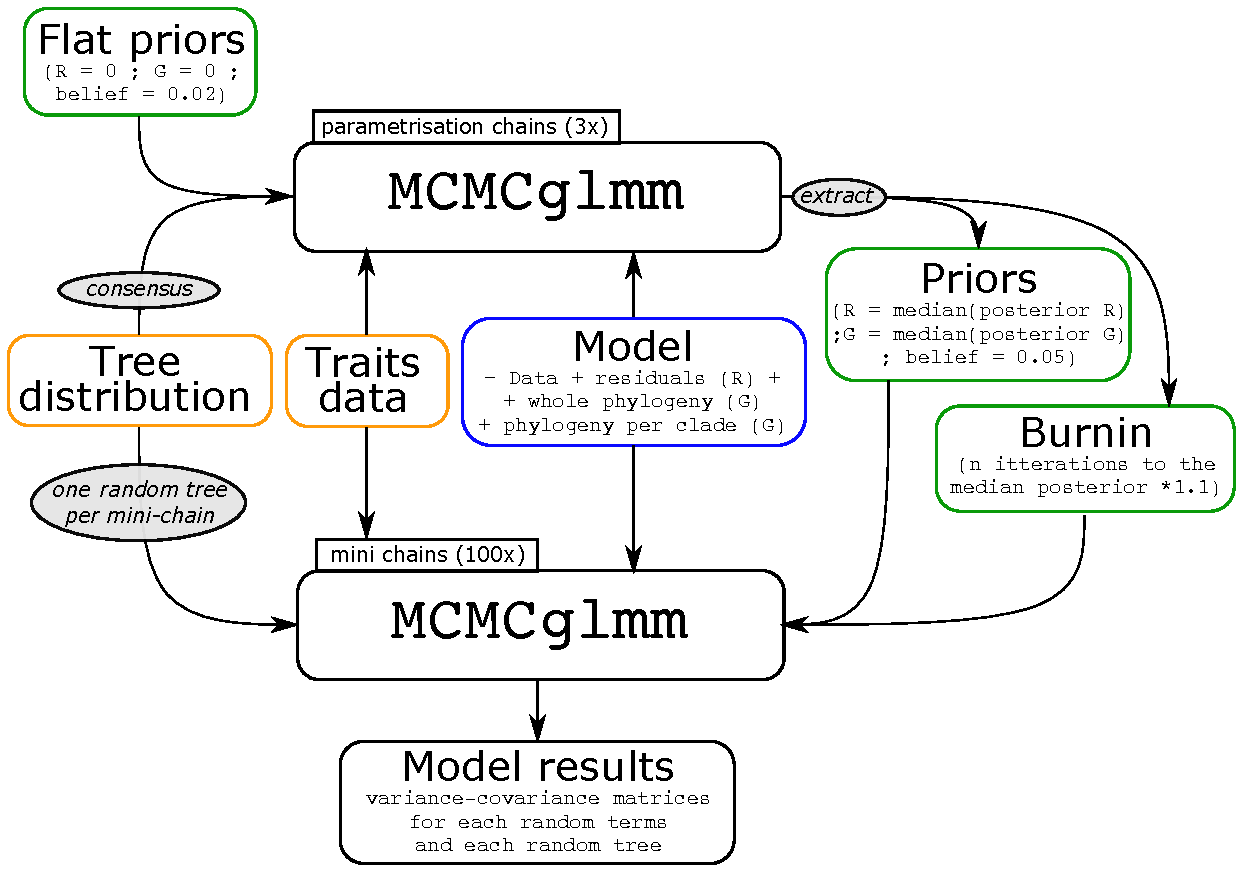
\includegraphics[width=0.9\textwidth]{Figures/mini-chains_diagram.pdf}
\caption{mcmcmcglmmm: mini-chains MCMCglmm method diagram. See Methods for more details.}
\label{Fig:mcmcmcglmm}
\end{figure}

\newpage

\begin{figure}[H]
\centering
   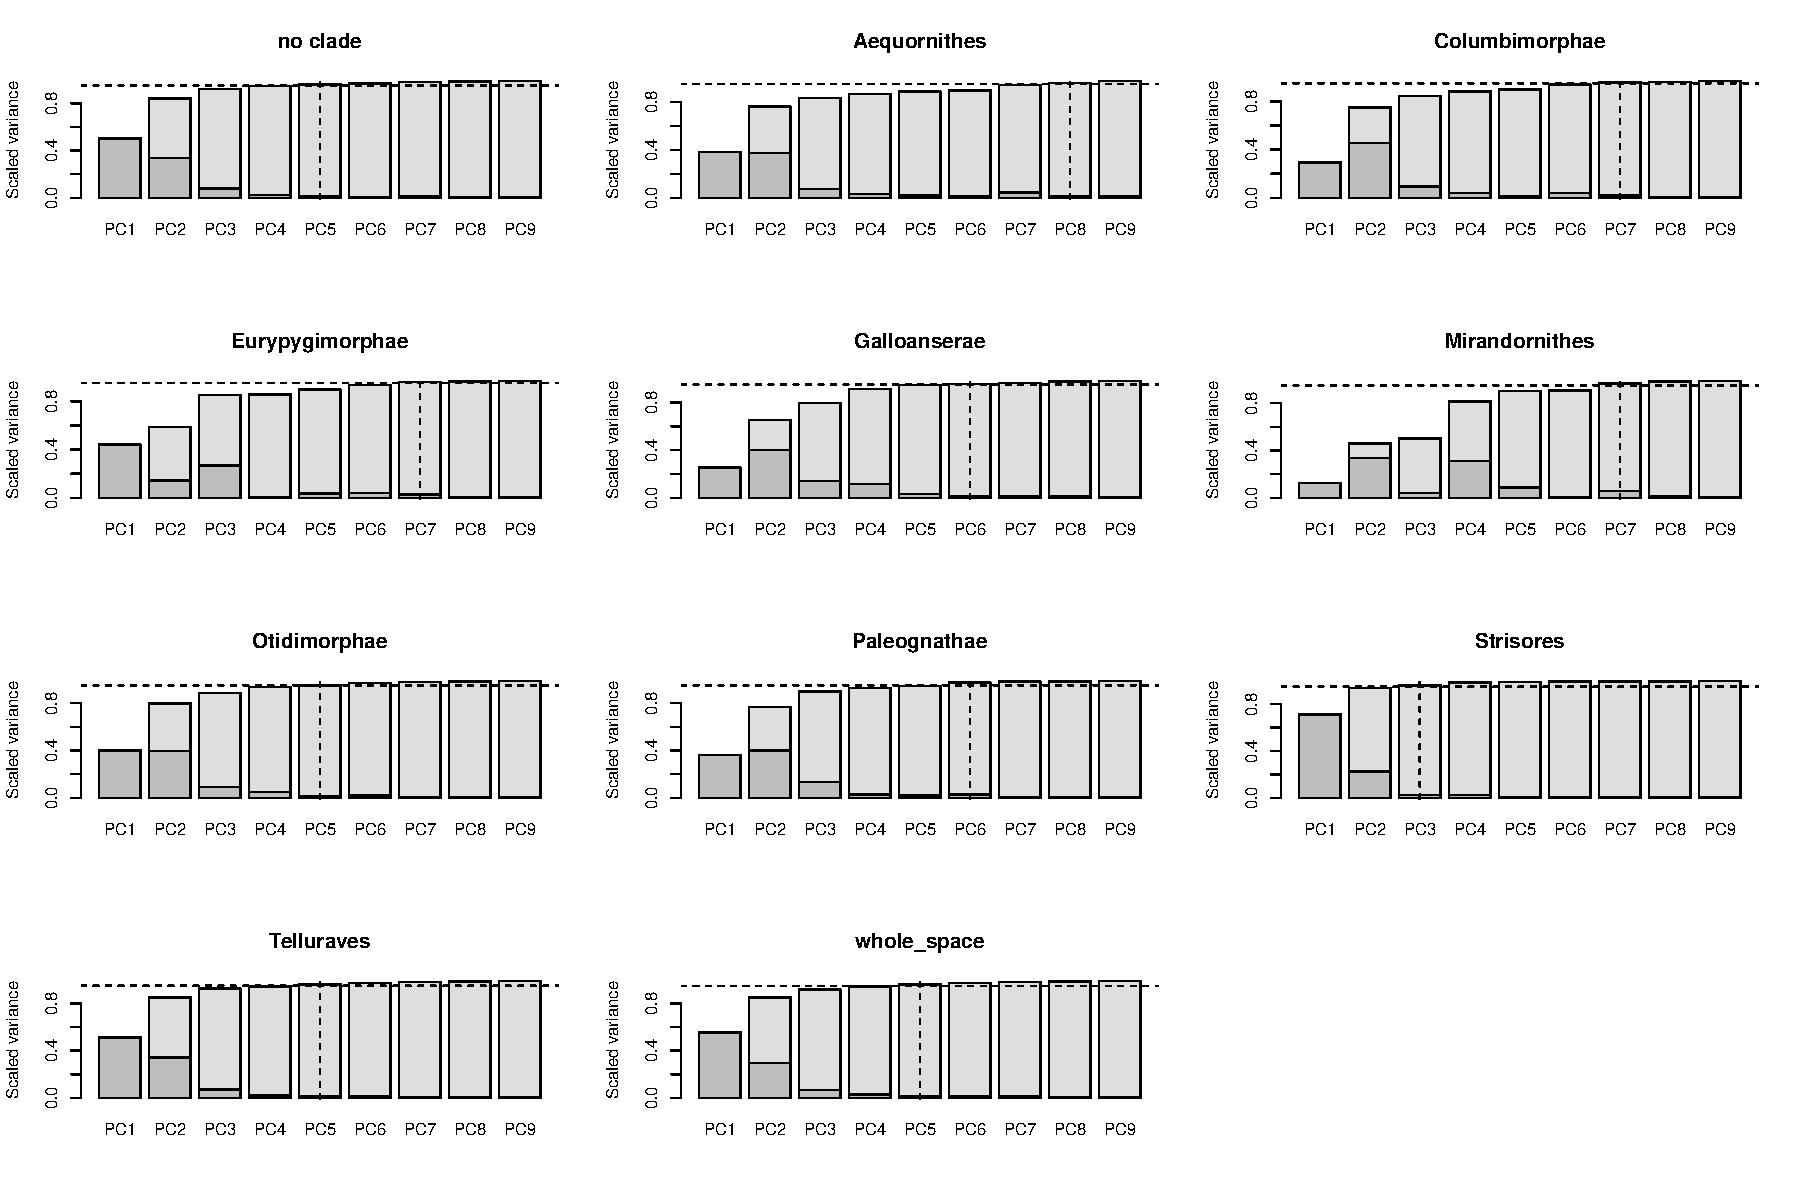
\includegraphics[width=0.9\textwidth]{Figures/axis_selection.pdf}
\caption{Variance and cumulative variance for each of the eight principal component (PC) axes for each super-order. Note that not all super-orders have their own variance explained matching the variance explained by the entire ordination. For example, Strisores only need the first three dimensions to explain at least 95\% of their variance within the shapespace whilst Aequornithes need all eight dimensions to achieve at least the same amount of variance explained. $no clade$ is the cumulative variance for species not present in the other displayed clades and $whole\_space$ is the cumulative for all species.}
\label{Fig:axes_variance}
\end{figure}

\newpage

\begin{figure}[H]
\centering
   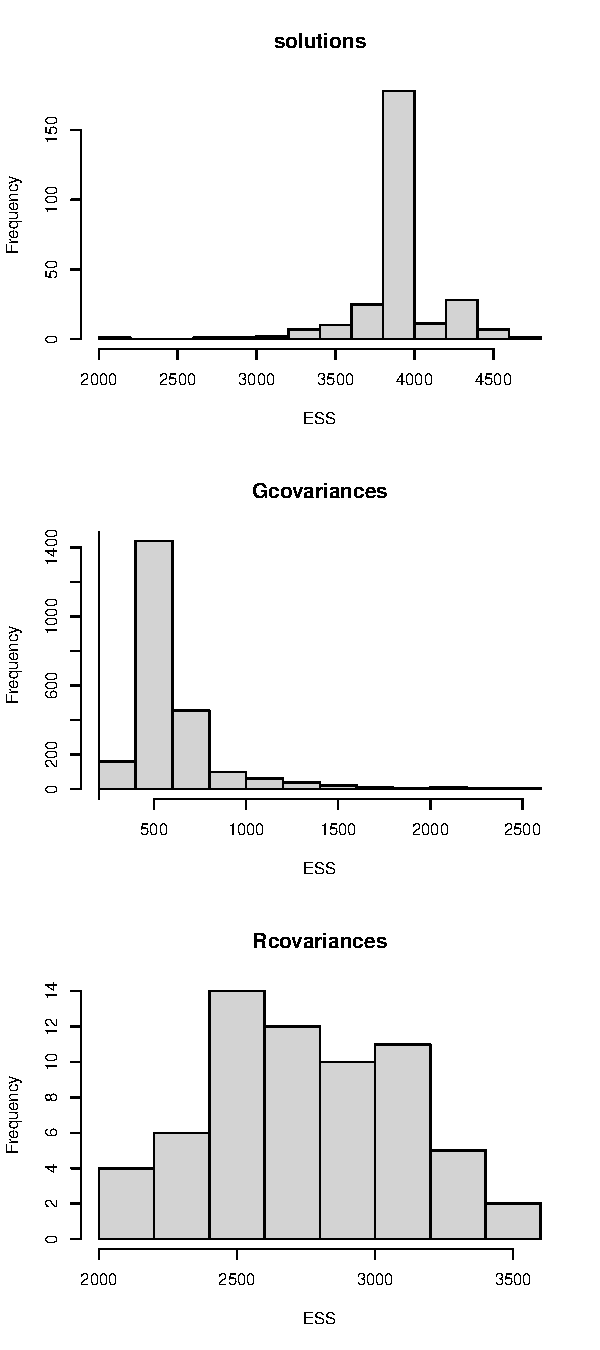
\includegraphics[width=0.5\textwidth]{Figures/parameters_ESS_all_birds.pdf}
\caption{Histogram of the effective sample sizes (ESS) for each class of parameters in the MCMCglmm model for all birds for the 4000 posteriors. \textbf{solutions} is the solution of the model; \textbf{Gcovariances} is the covariance for the random terms (the phylogeny and the clades); \textbf{Rcovariances} is the residual error term.}
\label{Fig:model_ess_all_birds}
\end{figure}

\newpage

\begin{figure}[H]
\centering
   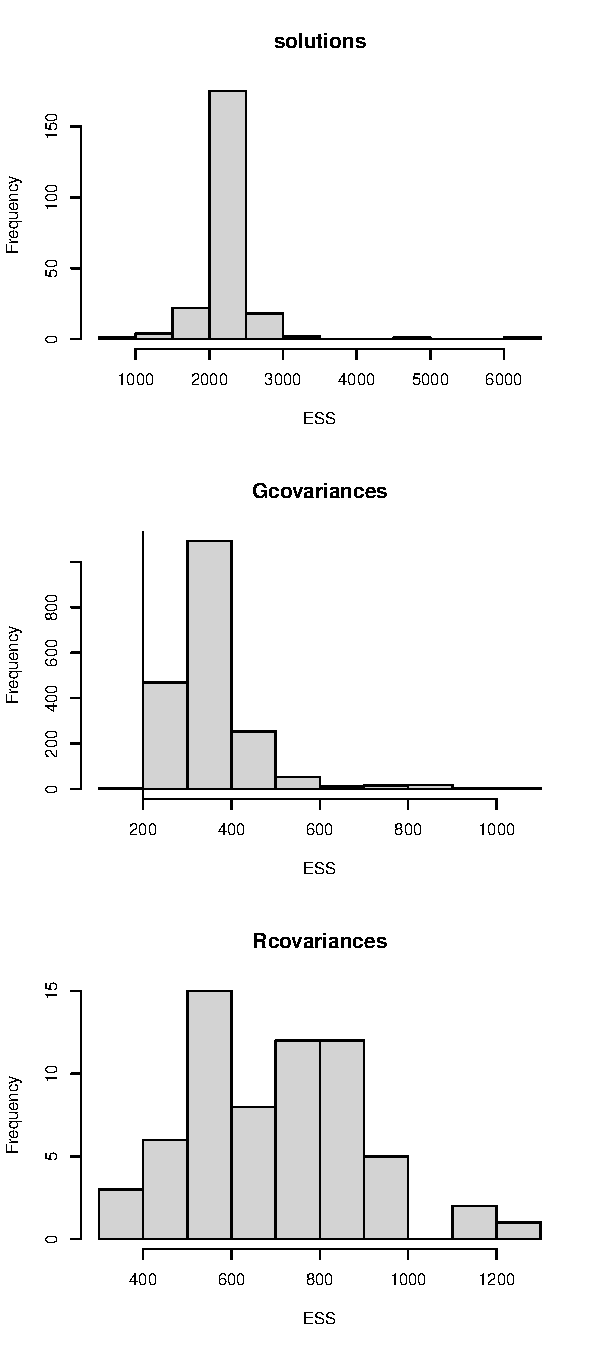
\includegraphics[width=0.5\textwidth]{Figures/parameters_ESS_passeriformes.pdf}
\caption{Histogram of the effective sample sizes (ESS) for each class of parameters in the MCMCglmm model for the Passeriformes for the 4000 posteriors. \textbf{solutions} is the solution of the model; \textbf{Gcovariances} is the covariance for the random terms (the phylogeny and the clades); \textbf{Rcovariances} is the residual error term.}
\label{Fig:model_ess_passeriformes}
\end{figure}

%---------------------------------------------
%
%   additional results
%
%---------------------------------------------

\newpage
\section{Additional results}
\subsection{Elaboration and innovation at the super-order or clade-wide phylogenetic level}

\begin{figure}[H]
\centering
   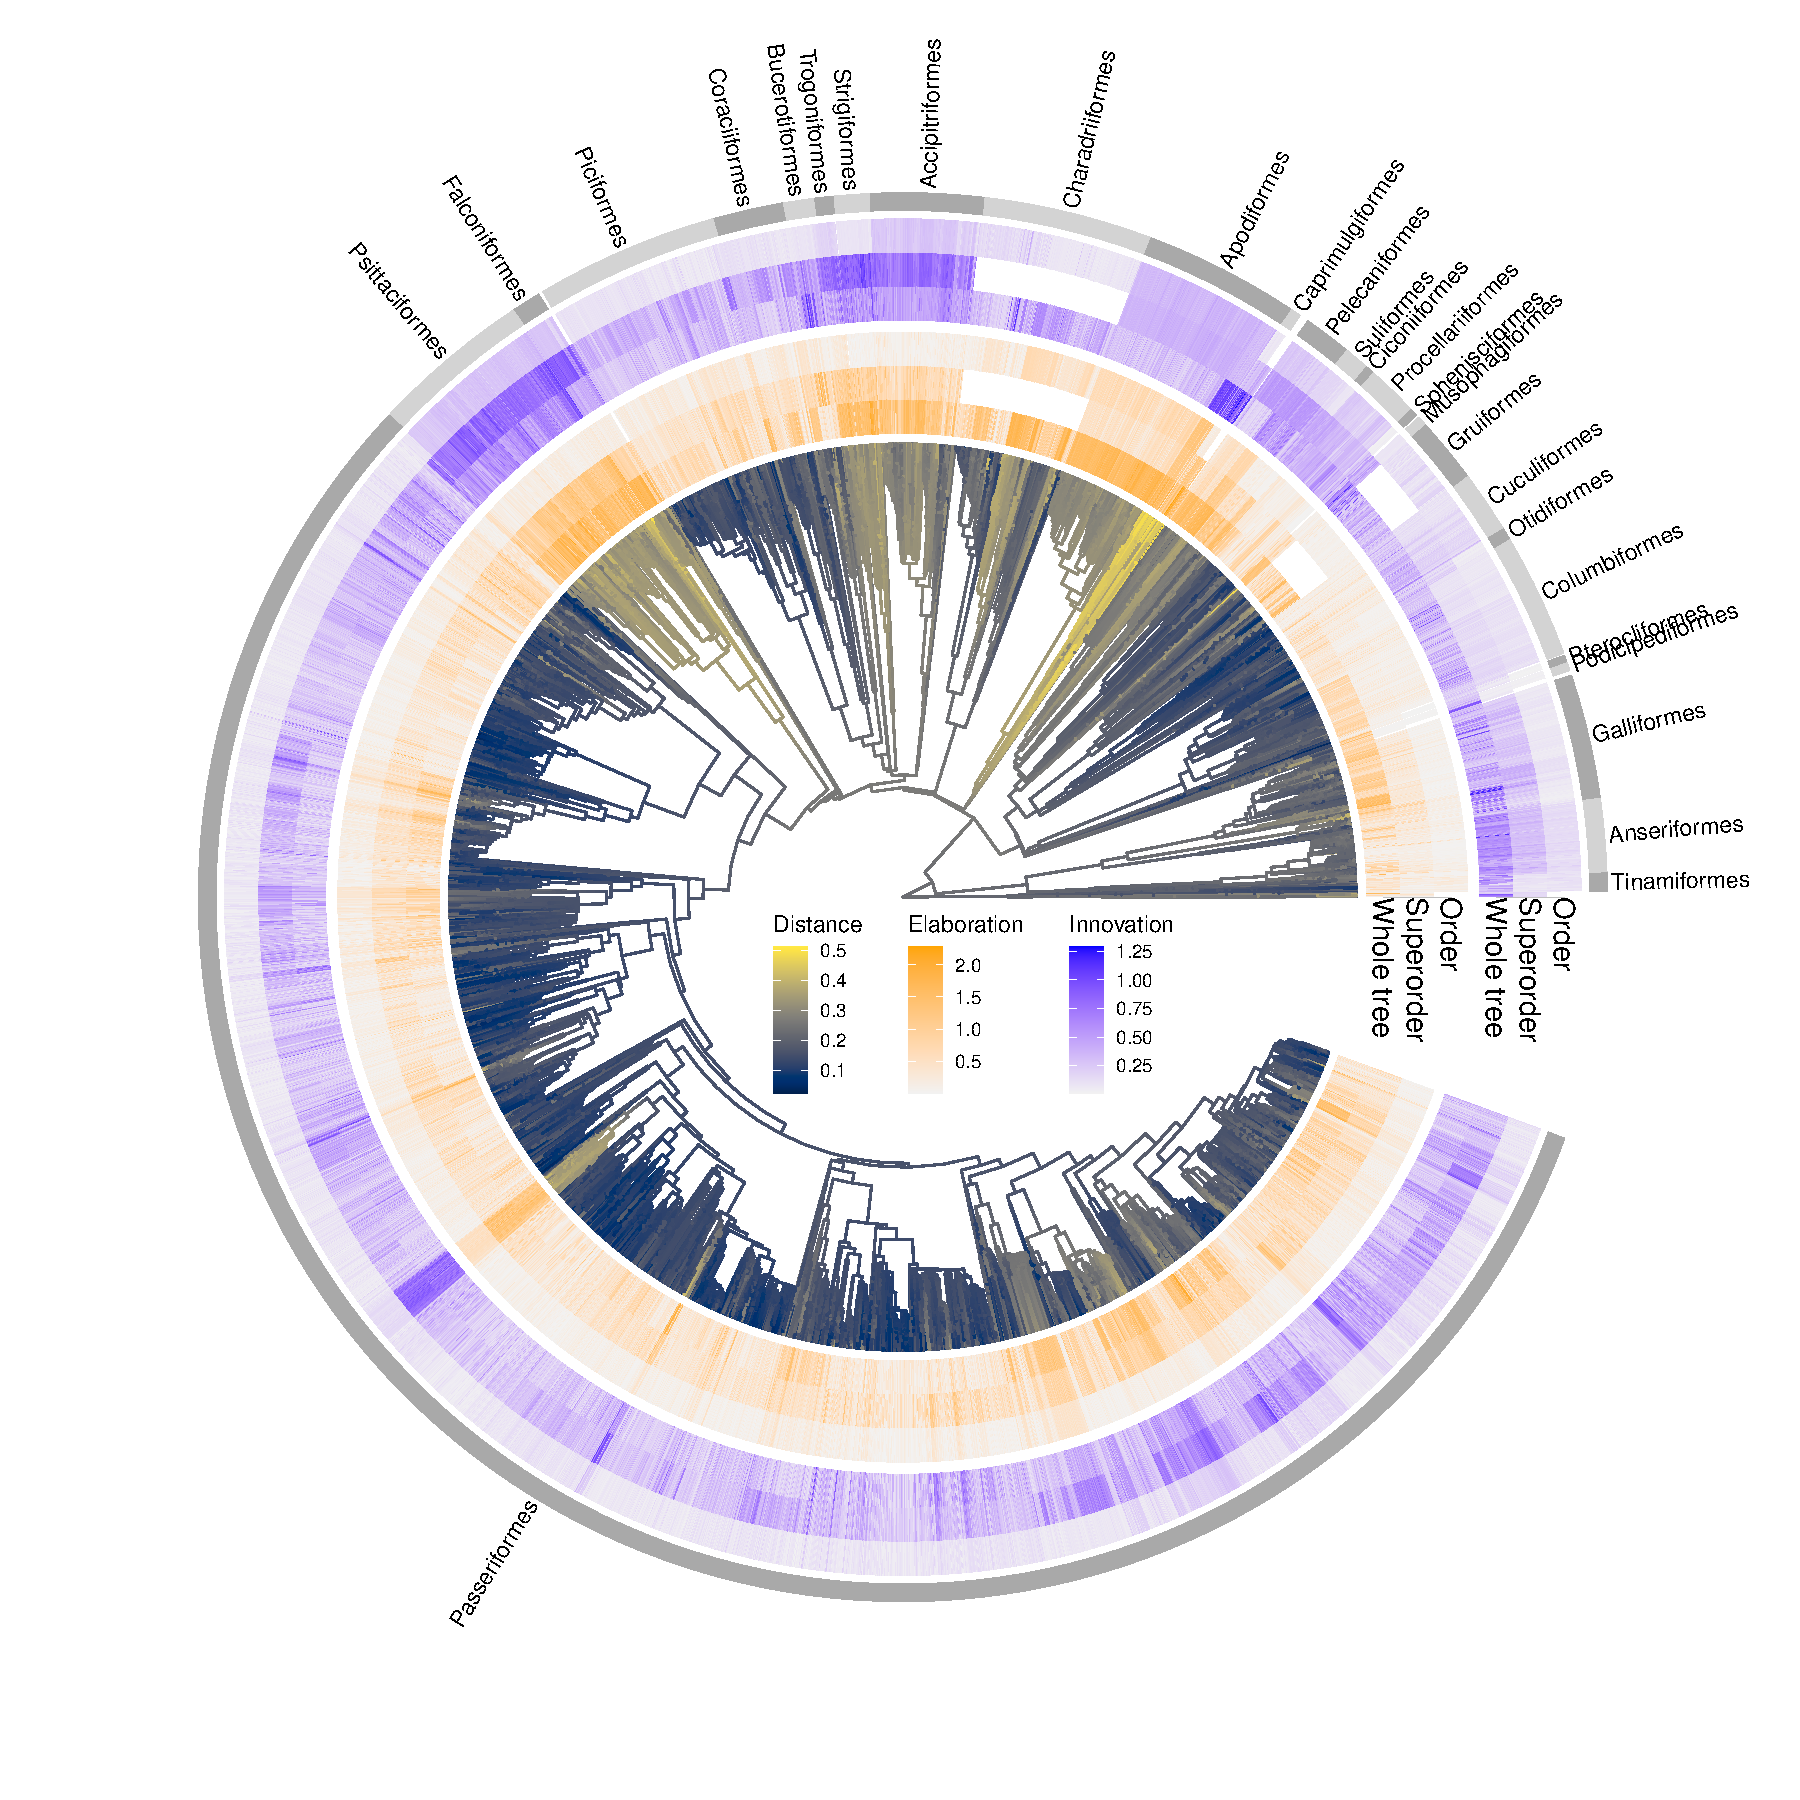
\includegraphics[width=0.7\textwidth]{Figures/InnovElabTree_supp_revision.pdf}
\caption{Avian phylogeny (n = 8748 species) showing Euclidean distance of species to the centroid of beak space (branches, cividis scale), and distributions of species beak shape $elaboration_{species}$ (inner circle, orange scale), and $innovation_{species}$ (outer circle, blue scale). Elaboration and innovation scores represent comparisons of species at the order, super-order and class-wide phylogenetic level.}
\label{Fig:phylogeny_supplement}
\end{figure}

%\newpage


\subsection{Correlations between $elaboration_{species}$ and $innovation_{species}$}

\begin{figure}[H]
\centering
   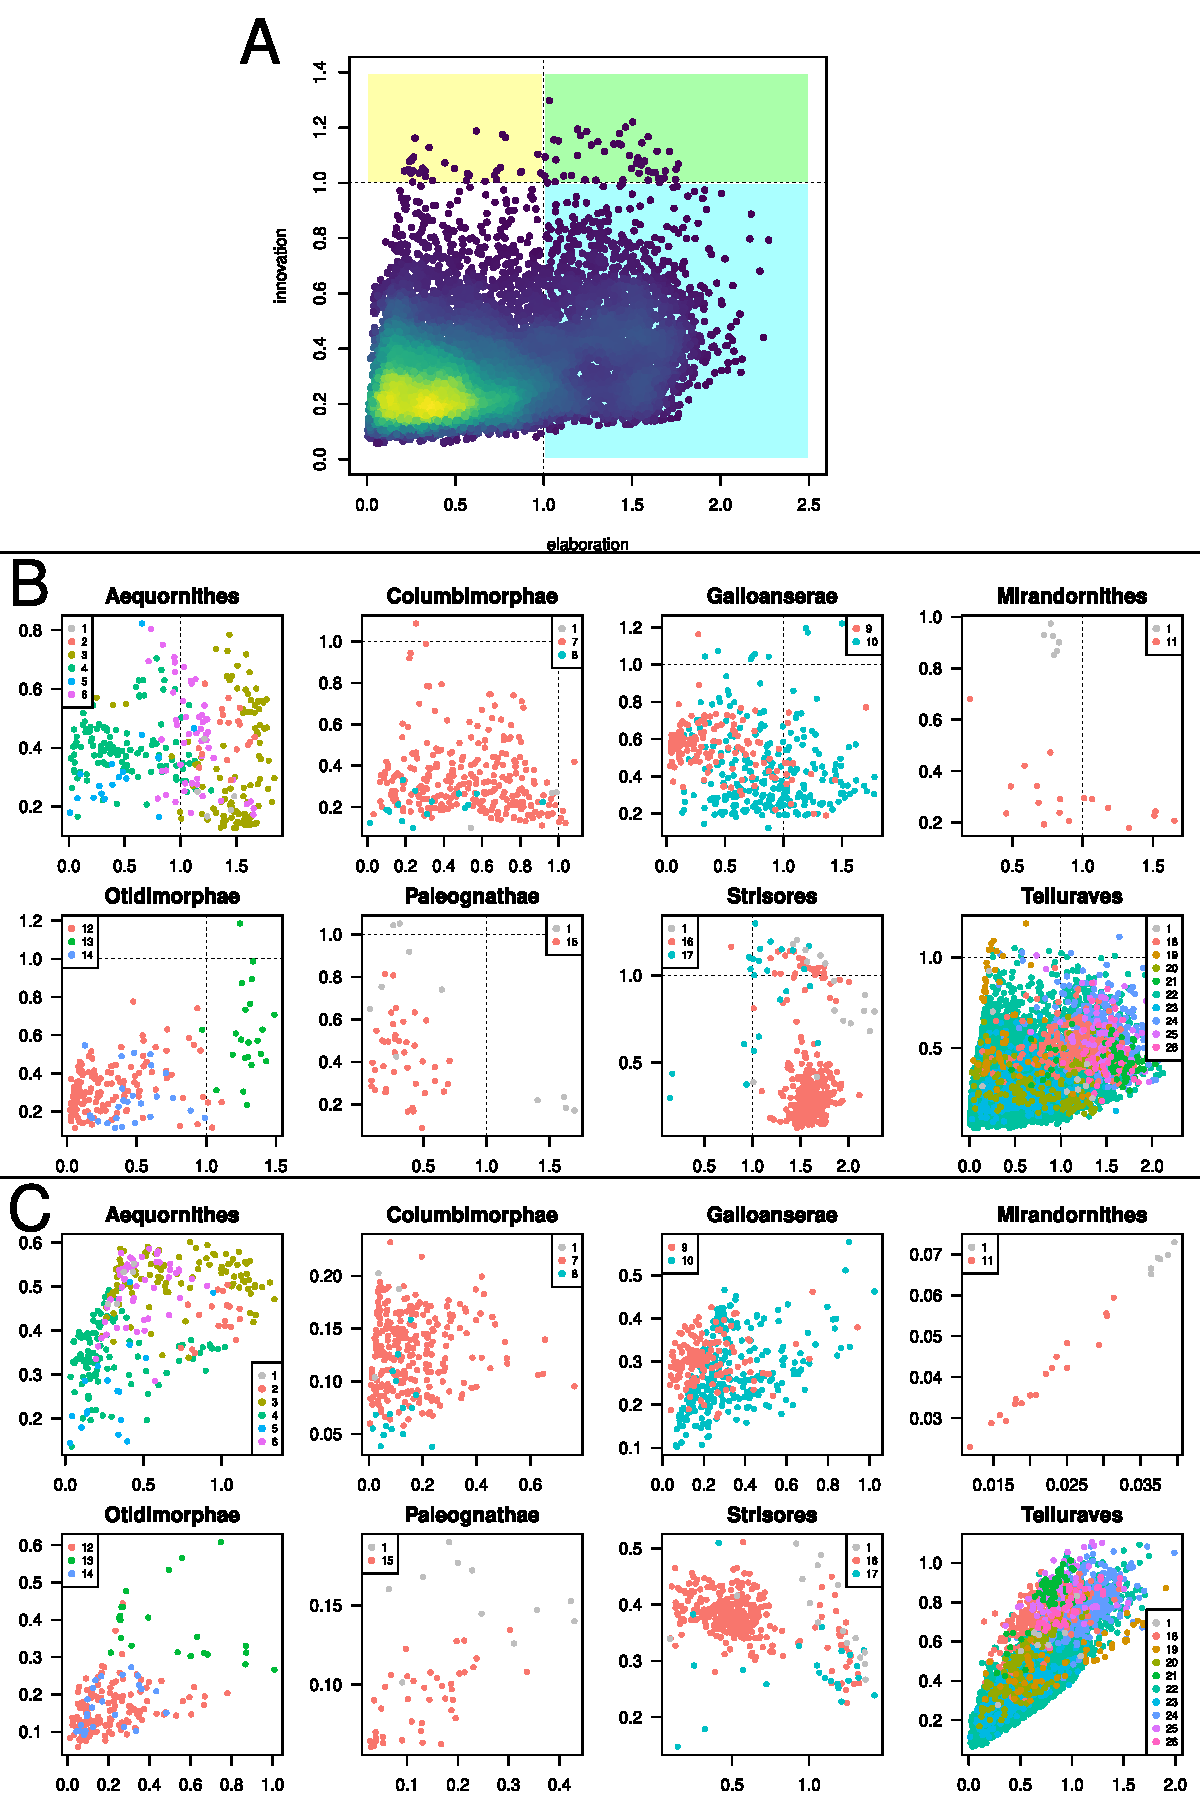
\includegraphics[width=0.5\textwidth]{Figures/correlations.pdf}
\caption{Median correlation plots of $elaboration_{species}$ and $innovation_{species}$ at different scales. 
\textbf{(A)} Correlation between $elaboration_{species}$ and $innovation_{species}$ for each species when projected on the whole phylogeny. 
The colours of the dots correspond to their density in the plot. 
Blue and yellow colours corresponds to respectively low and high density of species. 
The coloured quadrant in the background corresponds to $elaboration_{species}$ and $innovation_{species}$ scores higher than 1. 
The blue and yellow quadrants shows species with noticeably high $elaboration_{species}$ and $innovation_{species}$ respectively. 
The species in the green quadrant have noticeably high levels of both $elaboration_{species}$ and $innovation_{species}$.
\textbf{(B)} Correlation between $elaboration_{species}$ and $innovation_{species}$ for each species when projected on the whole phylogeny (mega-level projection) but plotted by super-order and coloured by order (see list below).
\textbf{C} correlation between $elaboration_{species}$ and $innovation_{species}$ for each species when projected on their super-orders' major axis of variation (macro-level projection). 
The colours correspond to each order. 
For the distribution of correlation scores, see Fig. \ref{Fig:fable_correlations}. 
The group numbers are:
1) others (groups with $<$ 15 species)
2) Corvoidea;
3) Malaconotoidea;
4) Orioloidea;
5) Meliphagoidea;
6) Bombycilloidea;
7) Muscicapoidea;
8) Emberizoidea;
9) Motacillidae;
10) Nectariniidae;
11) Passeridae;
12) PloceidaeEstrildidae;
13) Eurylaimides;
14) Furnariida;
15) Tyrannida;
16) Aegithaloidea;
17) Cisticolidae;
18) Fringillidae;
19) Hirundinidae;
20) Locustelloidea;
21) Paridae;
22) Pycnonotidae;
23) Sylvioidea.}
\label{Fig:figure_correlations}
\end{figure}

\newpage

\begin{figure}[H]
\centering
   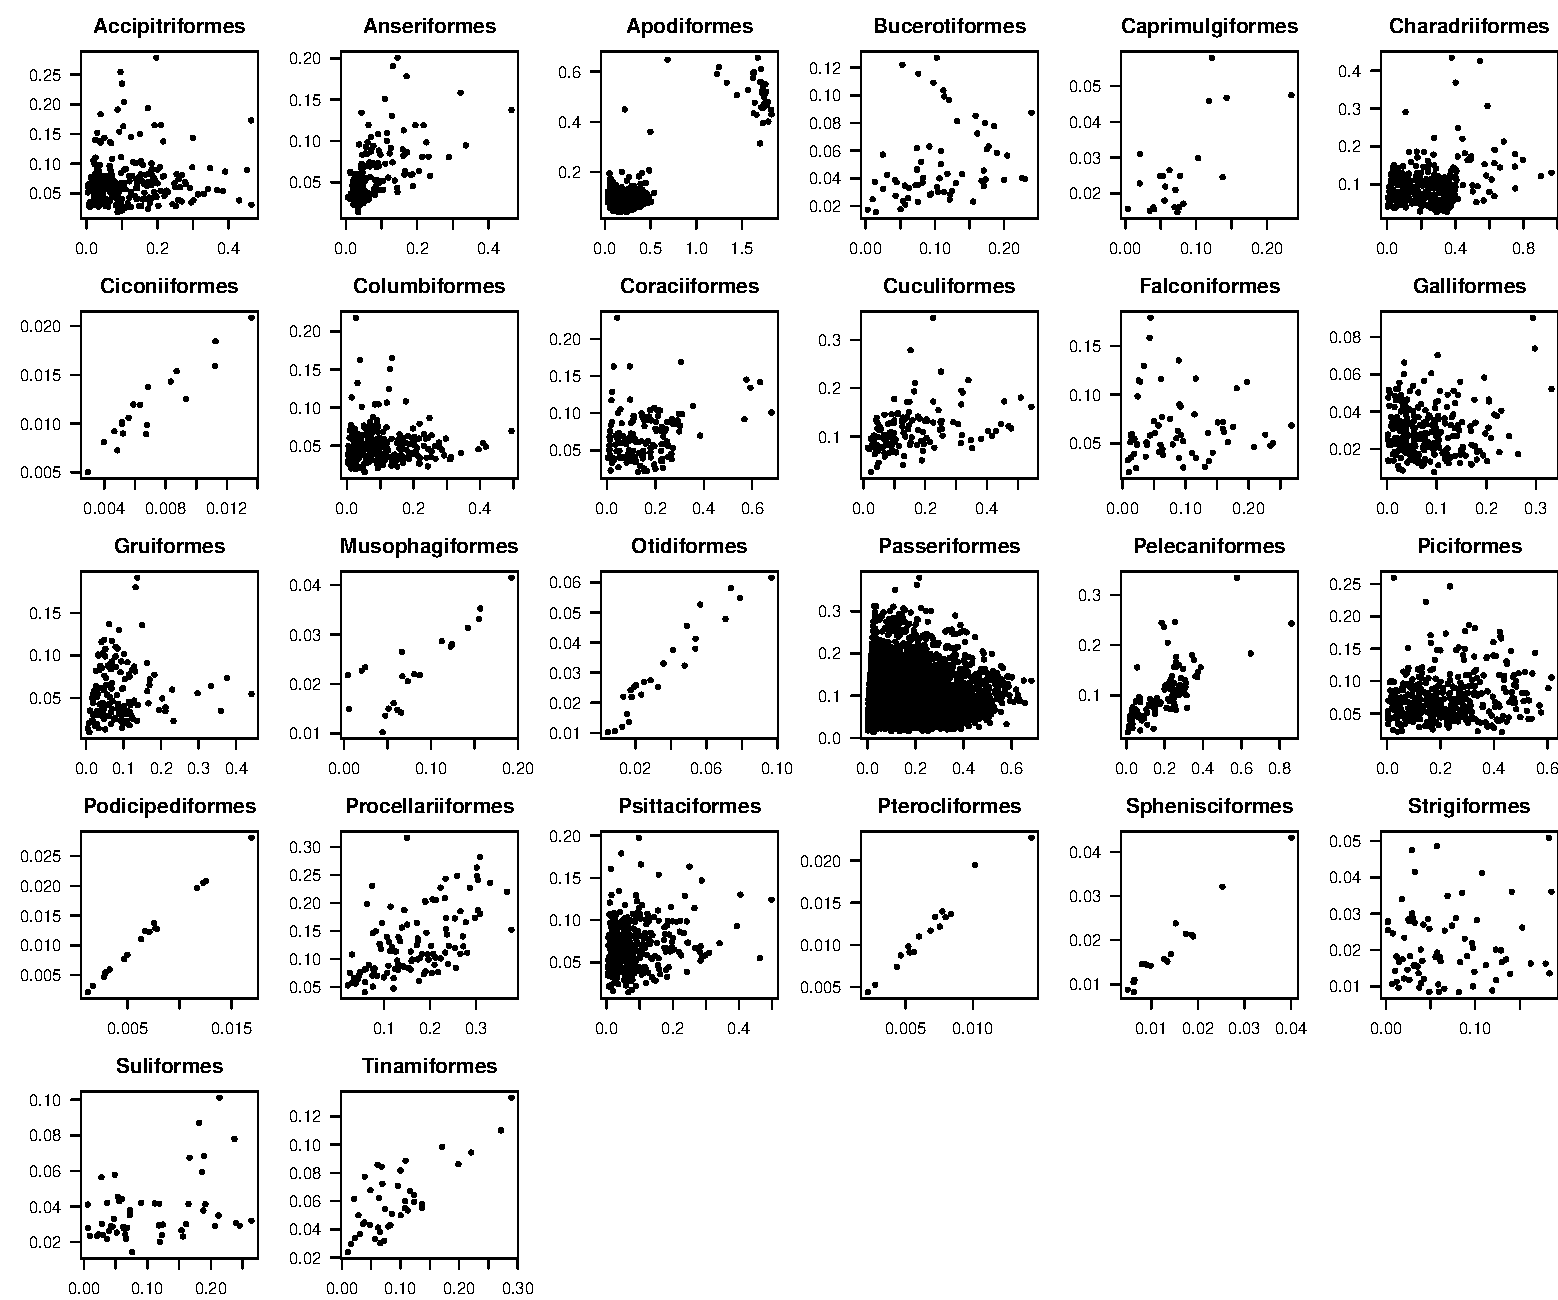
\includegraphics[width=0.9\textwidth]{Figures/correlations_2.pdf}
\caption{Median correlation plots of $elaboration_{species}$ and $innovation_{species}$ for each species projected on their order's phylogenetic major axis of beak variation. Each point is the median $elaboration_{species}$ and $innovation_{species}$ for one species from the distribution of 4000 posterior evolutionary rate matrices. The full distribution of the correlations between $elaboration_{species}$ and $innovation_{species}$ is available in the main text in Figure 3.}
\label{Fig:figure_correlations2}
\end{figure}

\newpage

\begin{figure}[H]
\centering
   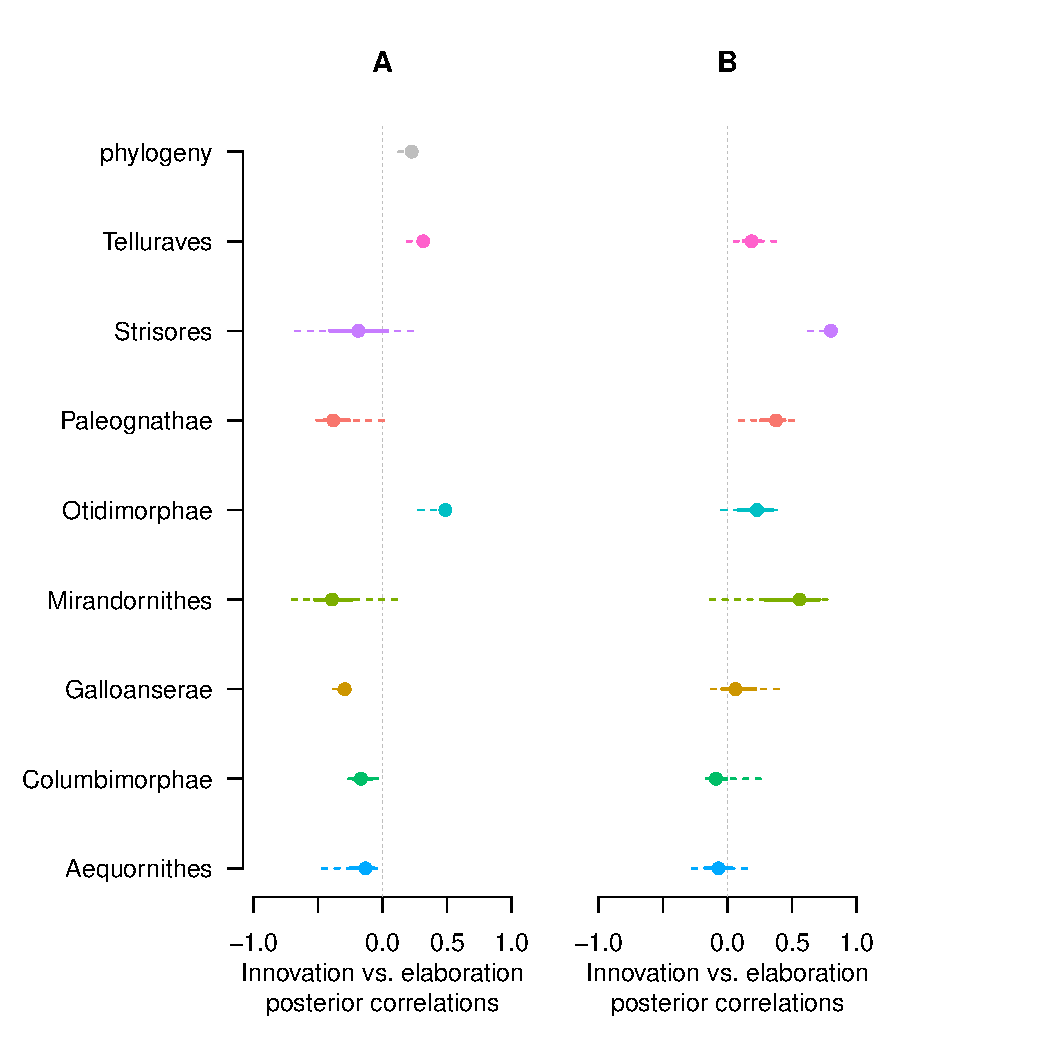
\includegraphics[width=0.9\textwidth]{Figures/correlations_fable_super_orders.pdf}
\caption{Posterior distributions of the correlation between $elaboration_{species}$ and $innovation_{species}$ for each super-orders in Fig. \ref{Fig:figure_correlations}.
A) Species' projection onto the class-wide phylogenetic major axes of beak variation (corresponding to the correlation scores in Fig. \ref{Fig:figure_correlations}A-B); B) Species' projection onto the super-orders' phylogenetic major axes of beak variation (corresponding to the correlation scores in Fig. \ref{Fig:figure_correlations}C).}
\label{Fig:fable_correlations_supplementary}
\end{figure}

\newpage

\begin{landscape}
% latex table generated in R 4.2.1 by xtable 1.8-4 package
% Thu Aug  4 16:49:31 2022
\begin{table}[ht]
\centering
\scriptsize
\begin{tabular}{llrrrrrrrr}
  \hline
Group & Comparison & n & ellipse sd & orthogonality & 2.5\% & 97.5\% & Post. prob. & 2.5\% & 97.5\% \\ 
  \hline
Aequornithes & phylogeny &  308 & 15.465 & 0.710 & 0.219 & 0.988 & 0.811 & 0.802 & 0.818 \\ 
  Columbimorphae & phylogeny &  285 & 5.916 & 0.884 & 0.564 & 0.995 & 0.998 & 0.997 & 0.999 \\ 
  Galloanserae & phylogeny &  421 & 13.489 & 0.800 & 0.369 & 0.992 & 0.832 & 0.826 & 0.838 \\ 
  Mirandornithes & phylogeny &   24 & 20.870 & 0.839 & 0.448 & 0.992 & 0.496 & 0.489 & 0.505 \\ 
  Otidimorphae & phylogeny &  181 & 16.800 & 0.680 & 0.291 & 0.983 & 0.795 & 0.788 & 0.802 \\ 
  Paleognathae & phylogeny &   52 & 20.728 & 0.718 & 0.264 & 0.985 & 0.803 & 0.797 & 0.810 \\ 
  Strisores & phylogeny &  370 & 16.237 & 0.787 & 0.469 & 0.986 & 0.992 & 0.990 & 0.994 \\ 
  Telluraves & phylogeny & 6604 & 14.339 & 0.730 & 0.294 & 0.988 & 0.662 & 0.655 & 0.672 \\ 
  Accipitriformes & phylogeny &  240 & 5.044 & 0.906 & 0.706 & 0.996 & 1.000 & 1.000 & 1.000 \\ 
  Anseriformes & phylogeny &  156 & 13.546 & 0.743 & 0.167 & 0.989 & 0.781 & 0.773 & 0.790 \\ 
  Apodiformes & phylogeny &  331 & 18.307 & 0.684 & 0.326 & 0.971 & 0.887 & 0.881 & 0.894 \\ 
  Bucerotiformes & phylogeny &   66 & 4.651 & 0.857 & 0.542 & 0.993 & 0.983 & 0.980 & 0.985 \\ 
  Caprimulgiformes & phylogeny &   23 & 11.555 & 0.847 & 0.533 & 0.992 & 0.938 & 0.934 & 0.943 \\ 
  Charadriiformes & phylogeny &  359 & 5.632 & 0.331 & 0.148 & 0.592 & 0.915 & 0.909 & 0.920 \\ 
  Ciconiiformes & phylogeny &   19 & 20.915 & 0.839 & 0.459 & 0.992 & 0.519 & 0.509 & 0.528 \\ 
  Columbiformes & phylogeny &  266 & 3.975 & 0.896 & 0.649 & 0.996 & 1.000 & 1.000 & 1.000 \\ 
  Coraciiformes & phylogeny &  149 & 17.618 & 0.358 & 0.196 & 0.603 & 0.980 & 0.976 & 0.983 \\ 
  Cuculiformes & phylogeny &  134 & 18.927 & 0.603 & 0.217 & 0.970 & 0.753 & 0.746 & 0.761 \\ 
  Falconiformes & phylogeny &   63 & 12.521 & 0.851 & 0.520 & 0.993 & 0.979 & 0.977 & 0.982 \\ 
  Galliformes & phylogeny &  265 & 1.416 & 0.894 & 0.694 & 0.995 & 1.000 & 1.000 & 1.000 \\ 
  Gruiformes & phylogeny &  138 & 7.922 & 0.543 & 0.215 & 0.894 & 0.948 & 0.944 & 0.953 \\ 
  Musophagiformes & phylogeny &   22 & 11.601 & 0.898 & 0.581 & 0.996 & 0.922 & 0.916 & 0.927 \\ 
  Otidiformes & phylogeny &   25 & 17.148 & 0.706 & 0.271 & 0.983 & 0.482 & 0.473 & 0.490 \\ 
  Passeriformes & phylogeny & 5229 & 11.642 & 0.428 & 0.189 & 0.650 & 1.000 & 0.999 & 1.000 \\ 
  Pelecaniformes & phylogeny &  103 & 28.435 & 0.537 & 0.284 & 0.937 & 0.747 & 0.741 & 0.755 \\ 
  Piciformes & phylogeny &  390 & 15.366 & 0.460 & 0.216 & 0.684 & 1.000 & 0.999 & 1.000 \\ 
  Podicipediformes & phylogeny &   18 & 20.335 & 0.828 & 0.453 & 0.993 & 0.491 & 0.482 & 0.500 \\ 
  Procellariiformes & phylogeny &  112 & 13.408 & 0.529 & 0.241 & 0.949 & 0.608 & 0.600 & 0.617 \\ 
  Psittaciformes & phylogeny &  341 & 12.975 & 0.572 & 0.433 & 0.755 & 1.000 & 1.000 & 1.000 \\ 
  Pterocliformes & phylogeny &   16 & 21.382 & 0.834 & 0.459 & 0.994 & 0.507 & 0.500 & 0.518 \\ 
  Sphenisciformes & phylogeny &   17 & 21.149 & 0.809 & 0.415 & 0.991 & 0.501 & 0.490 & 0.509 \\ 
  Strigiformes & phylogeny &   76 & 2.241 & 0.921 & 0.721 & 0.996 & 1.000 & 1.000 & 1.000 \\ 
  Suliformes & phylogeny &   52 & 7.537 & 0.745 & 0.437 & 0.976 & 0.994 & 0.993 & 0.996 \\ 
  Tinamiformes & phylogeny &   41 & 18.518 & 0.805 & 0.331 & 0.991 & 0.721 & 0.711 & 0.729 \\ 
  Trogoniformes & phylogeny &   41 & 9.463 & 0.882 & 0.593 & 0.995 & 0.997 & 0.996 & 0.999 \\ 
  Procellariiformes & Aequornithes &  112 & 13.408 & 0.677 & 0.263 & 0.986 & 0.699 & 0.690 & 0.707 \\ 
  Sphenisciformes & Aequornithes &   17 & 21.149 & 0.744 & 0.348 & 0.988 & 0.414 & 0.406 & 0.423 \\ 
  Ciconiiformes & Aequornithes &   19 & 20.915 & 0.790 & 0.365 & 0.987 & 0.436 & 0.426 & 0.444 \\ 
  Pelecaniformes & Aequornithes &  103 & 28.435 & 0.541 & 0.196 & 0.968 & 0.675 & 0.666 & 0.683 \\ 
  Suliformes & Aequornithes &   52 & 7.537 & 0.299 & 0.128 & 0.875 & 0.761 & 0.754 & 0.769 \\ 
  Columbiformes & Columbimorphae &  266 & 3.975 & 0.182 & 0.079 & 0.424 & 0.638 & 0.630 & 0.647 \\ 
  Pterocliformes & Columbimorphae &   16 & 21.382 & 0.801 & 0.396 & 0.993 & 0.464 & 0.454 & 0.473 \\ 
  Galliformes & Galloanserae &  265 & 1.416 & 0.327 & 0.146 & 0.905 & 1.000 & 1.000 & 1.000 \\ 
  Anseriformes & Galloanserae &  156 & 13.546 & 0.499 & 0.206 & 0.963 & 0.599 & 0.591 & 0.606 \\ 
  Podicipediformes & Mirandornithes &   18 & 20.335 & 0.552 & 0.170 & 0.972 & 0.492 & 0.483 & 0.500 \\ 
  Otidiformes & Otidimorphae &   25 & 17.148 & 0.608 & 0.208 & 0.980 & 0.397 & 0.390 & 0.406 \\ 
  Cuculiformes & Otidimorphae &  134 & 18.927 & 0.486 & 0.173 & 0.959 & 0.517 & 0.510 & 0.527 \\ 
  Musophagiformes & Otidimorphae &   22 & 11.601 & 0.487 & 0.181 & 0.963 & 0.590 & 0.582 & 0.598 \\ 
  Tinamiformes & Paleognathae &   41 & 18.518 & 0.455 & 0.145 & 0.964 & 0.440 & 0.433 & 0.450 \\ 
  Caprimulgiformes & Strisores &   23 & 11.555 & 0.327 & 0.152 & 0.858 & 0.516 & 0.506 & 0.524 \\ 
  Apodiformes & Strisores &  331 & 18.307 & 0.340 & 0.141 & 0.797 & 0.529 & 0.519 & 0.536 \\ 
  Trogoniformes & Telluraves &   41 & 9.463 & 0.500 & 0.200 & 0.963 & 0.881 & 0.874 & 0.887 \\ 
  Bucerotiformes & Telluraves &   66 & 4.651 & 0.489 & 0.181 & 0.959 & 0.820 & 0.814 & 0.826 \\ 
  Coraciiformes & Telluraves &  149 & 17.618 & 0.676 & 0.343 & 0.983 & 0.999 & 0.998 & 1.000 \\ 
  Piciformes & Telluraves &  390 & 15.366 & 0.605 & 0.226 & 0.978 & 1.000 & 0.999 & 1.000 \\ 
  Strigiformes & Telluraves &   76 & 2.241 & 0.523 & 0.207 & 0.962 & 1.000 & 0.999 & 1.000 \\ 
  Accipitriformes & Telluraves &  240 & 5.044 & 0.482 & 0.169 & 0.961 & 0.976 & 0.974 & 0.980 \\ 
  Falconiformes & Telluraves &   63 & 12.521 & 0.523 & 0.206 & 0.964 & 0.839 & 0.831 & 0.846 \\ 
  Psittaciformes & Telluraves &  341 & 12.975 & 0.648 & 0.275 & 0.982 & 1.000 & 0.999 & 1.000 \\ 
  Passeriformes & Telluraves & 5229 & 11.642 & 0.634 & 0.274 & 0.980 & 1.000 & 1.000 & 1.000 \\ 
  Corvides & Passeriformes &  609 & 16.462 & 0.195 & 0.097 & 0.495 & 0.546 & 0.530 & 0.561 \\ 
  Meliphagoidea & Passeriformes &  214 & 19.362 & 0.248 & 0.120 & 0.832 & 0.524 & 0.509 & 0.542 \\ 
  Muscicapida & Passeriformes &  702 & 16.961 & 0.354 & 0.101 & 0.798 & 0.681 & 0.663 & 0.697 \\ 
  Passerida & Passeriformes & 1492 & 3.448 & 0.370 & 0.203 & 0.542 & 1.000 & 0.998 & 1.000 \\ 
  Suboscines & Passeriformes &  978 & 13.676 & 0.455 & 0.173 & 0.889 & 0.796 & 0.785 & 0.814 \\ 
  Sylviida & Passeriformes & 1131 & 16.555 & 0.474 & 0.128 & 0.947 & 0.527 & 0.510 & 0.548 \\ 
  Aegithaloidea & Passeriformes &  105 & 24.869 & 0.324 & 0.155 & 0.899 & 0.447 & 0.431 & 0.462 \\ 
  Bombycilloidea & Passeriformes &  112 & 10.938 & 0.404 & 0.179 & 0.728 & 0.834 & 0.818 & 0.850 \\ 
  Cisticolidae & Passeriformes &  141 & 14.966 & 0.459 & 0.173 & 0.905 & 0.519 & 0.504 & 0.533 \\ 
  Corvoidea & Passeriformes &  248 & 3.303 & 0.499 & 0.343 & 0.672 & 1.000 & 1.000 & 1.000 \\ 
  Emberizoidea & Passeriformes &  752 & 16.601 & 0.455 & 0.210 & 0.932 & 0.730 & 0.716 & 0.746 \\ 
  Eurylaimides & Passeriformes &   51 & 22.653 & 0.165 & 0.075 & 0.423 & 0.440 & 0.423 & 0.454 \\ 
  Fringillidae & Passeriformes &   87 & 3.730 & 0.428 & 0.198 & 0.751 & 0.926 & 0.914 & 0.938 \\ 
  Furnariida & Passeriformes &  488 & 6.684 & 0.384 & 0.198 & 0.640 & 0.904 & 0.892 & 0.915 \\ 
  Hirundinidae & Passeriformes &   77 & 10.776 & 0.691 & 0.447 & 0.967 & 0.950 & 0.942 & 0.957 \\ 
  Locustelloidea & Passeriformes &  106 & 22.109 & 0.339 & 0.117 & 0.892 & 0.481 & 0.465 & 0.497 \\ 
  Malaconotoidea & Passeriformes &  205 & 19.275 & 0.495 & 0.283 & 0.838 & 0.883 & 0.873 & 0.891 \\ 
  Meliphagoidea & Passeriformes &  214 & 19.362 & 0.239 & 0.106 & 0.741 & 0.524 & 0.504 & 0.545 \\ 
  Motacillidae & Passeriformes &   58 & 16.078 & 0.486 & 0.186 & 0.918 & 0.638 & 0.625 & 0.653 \\ 
  Muscicapoidea & Passeriformes &  576 & 17.136 & 0.318 & 0.113 & 0.624 & 0.763 & 0.751 & 0.778 \\ 
  Nectariniidae & Passeriformes &  166 & 19.789 & 0.222 & 0.109 & 0.427 & 0.651 & 0.638 & 0.669 \\ 
  Orioloidea & Passeriformes &   54 & 21.510 & 0.466 & 0.147 & 0.972 & 0.500 & 0.484 & 0.520 \\ 
  Paridae & Passeriformes &   69 & 8.747 & 0.559 & 0.275 & 0.851 & 0.937 & 0.927 & 0.943 \\ 
  Passeridae & Passeriformes &   39 & 19.891 & 0.525 & 0.146 & 0.969 & 0.418 & 0.405 & 0.433 \\ 
  Petroicidae & Passeriformes &   35 & 31.236 & 0.484 & 0.170 & 0.975 & 0.401 & 0.387 & 0.419 \\ 
  PloceidaeEstrildidae & Passeriformes &  261 & 6.009 & 0.896 & 0.627 & 0.995 & 1.000 & 0.999 & 1.000 \\ 
  Pycnonotidae & Passeriformes &  123 & 17.818 & 0.229 & 0.117 & 0.581 & 0.521 & 0.506 & 0.540 \\ 
  Sylvioidea & Passeriformes &  403 & 12.158 & 0.405 & 0.157 & 0.944 & 0.572 & 0.557 & 0.589 \\ 
  Tyrannida & Passeriformes &  439 & 26.513 & 0.466 & 0.181 & 0.936 & 0.586 & 0.570 & 0.607 \\ 
  Orioloidea & Corvides &   54 & 21.510 & 0.502 & 0.150 & 0.968 & 0.487 & 0.469 & 0.502 \\ 
  Corvoidea & Corvides &  248 & 3.303 & 0.464 & 0.171 & 0.761 & 0.995 & 0.990 & 0.998 \\ 
  Malaconotoidea & Corvides &  205 & 19.275 & 0.556 & 0.283 & 0.893 & 0.892 & 0.881 & 0.903 \\ 
  Bombycilloidea & Muscicapida &  112 & 10.938 & 0.260 & 0.093 & 0.742 & 0.572 & 0.550 & 0.593 \\ 
  Muscicapoidea & Muscicapida &  576 & 17.136 & 0.271 & 0.085 & 0.796 & 0.578 & 0.553 & 0.591 \\ 
  Nectariniidae & Passerida &  166 & 19.789 & 0.464 & 0.278 & 0.719 & 0.960 & 0.952 & 0.967 \\ 
  PloceidaeEstrildidae & Passerida &  261 & 6.009 & 0.605 & 0.369 & 0.834 & 0.991 & 0.986 & 0.995 \\ 
  Emberizoidea & Passerida &  752 & 16.601 & 0.765 & 0.271 & 0.984 & 0.885 & 0.875 & 0.898 \\ 
  Motacillidae & Passerida &   58 & 16.078 & 0.756 & 0.239 & 0.987 & 0.823 & 0.810 & 0.839 \\ 
  Passeridae & Passerida &   39 & 19.891 & 0.668 & 0.225 & 0.986 & 0.524 & 0.506 & 0.540 \\ 
  Eurylaimides & Suboscines &   51 & 22.653 & 0.495 & 0.222 & 0.928 & 0.909 & 0.895 & 0.922 \\ 
  Tyrannida & Suboscines &  439 & 26.513 & 0.404 & 0.134 & 0.956 & 0.479 & 0.458 & 0.494 \\ 
  Furnariida & Suboscines &  488 & 6.684 & 0.245 & 0.100 & 0.764 & 0.695 & 0.679 & 0.709 \\ 
  Paridae & Sylviida &   69 & 8.747 & 0.388 & 0.151 & 0.934 & 0.788 & 0.771 & 0.802 \\ 
  Locustelloidea & Sylviida &  106 & 22.109 & 0.483 & 0.168 & 0.930 & 0.664 & 0.646 & 0.682 \\ 
  Aegithaloidea & Sylviida &  105 & 24.869 & 0.530 & 0.177 & 0.967 & 0.642 & 0.626 & 0.661 \\ 
  Hirundinidae & Sylviida &   77 & 10.776 & 0.522 & 0.272 & 0.956 & 0.857 & 0.842 & 0.867 \\ 
  Pycnonotidae & Sylviida &  123 & 17.818 & 0.558 & 0.172 & 0.979 & 0.842 & 0.830 & 0.860 \\ 
  Sylvioidea & Sylviida &  403 & 12.158 & 0.444 & 0.132 & 0.963 & 0.575 & 0.557 & 0.593 \\ 
  Cisticolidae & Sylviida &  141 & 14.966 & 0.477 & 0.145 & 0.955 & 0.531 & 0.516 & 0.553 \\ 
  Fringillidae & Sylviida &   87 & 3.730 & 0.718 & 0.179 & 0.988 & 0.964 & 0.955 & 0.973 \\ 
   \hline
\end{tabular}
\caption{Posterior variance-covariance ellipses results for each clade compared to their parent clade or their parent parents clade (Comparison). n = the number of species per group. sd = the standard deviation of the ellipses orientation (across the posterior distribution). orthogonality = the degree of right angle for each group compared to their parent or parent's group (0 = parellel, 1 = orthogonal). Post. prob = the posterior probability of the orthogonality in the focal group being different from the comparison one (the 95\% CI is from the randomised posterior probabilities).} 
\label{tab_ortho_results}
\end{table}

\end{landscape}

\newpage

\subsection{Elaboration and innovation through time}


\begin{figure}[H]
\centering
   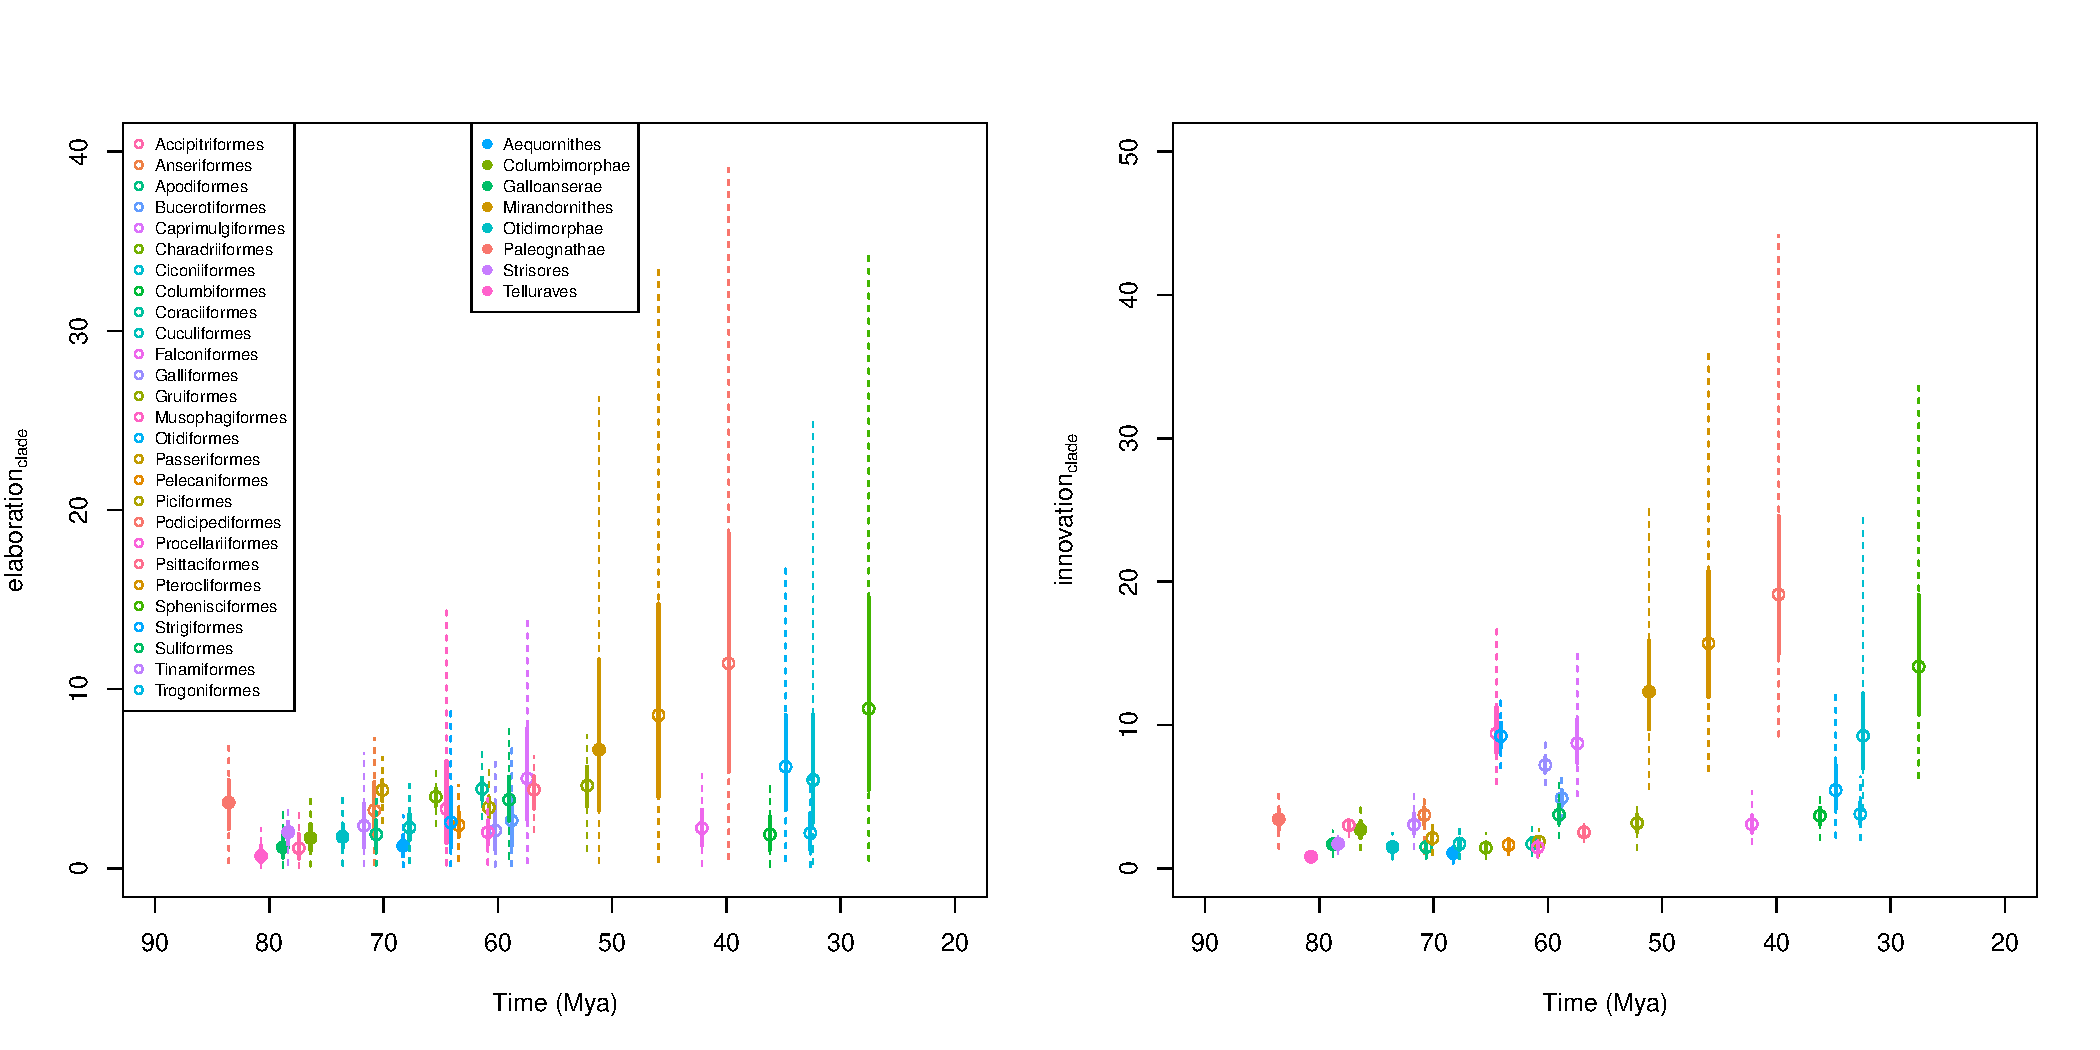
\includegraphics[width=1\textwidth]{Figures/Elaboration_and_innovation_clade_through_time.pdf}
\caption{Distribution of $elaboration_{clade}$ and $innovation_{clade}$ for each order and super-order through time in millions of years (Mya).}
\label{Fig:figure_ei_clade_through_time}
\end{figure}


\begin{figure}[H]
\centering
   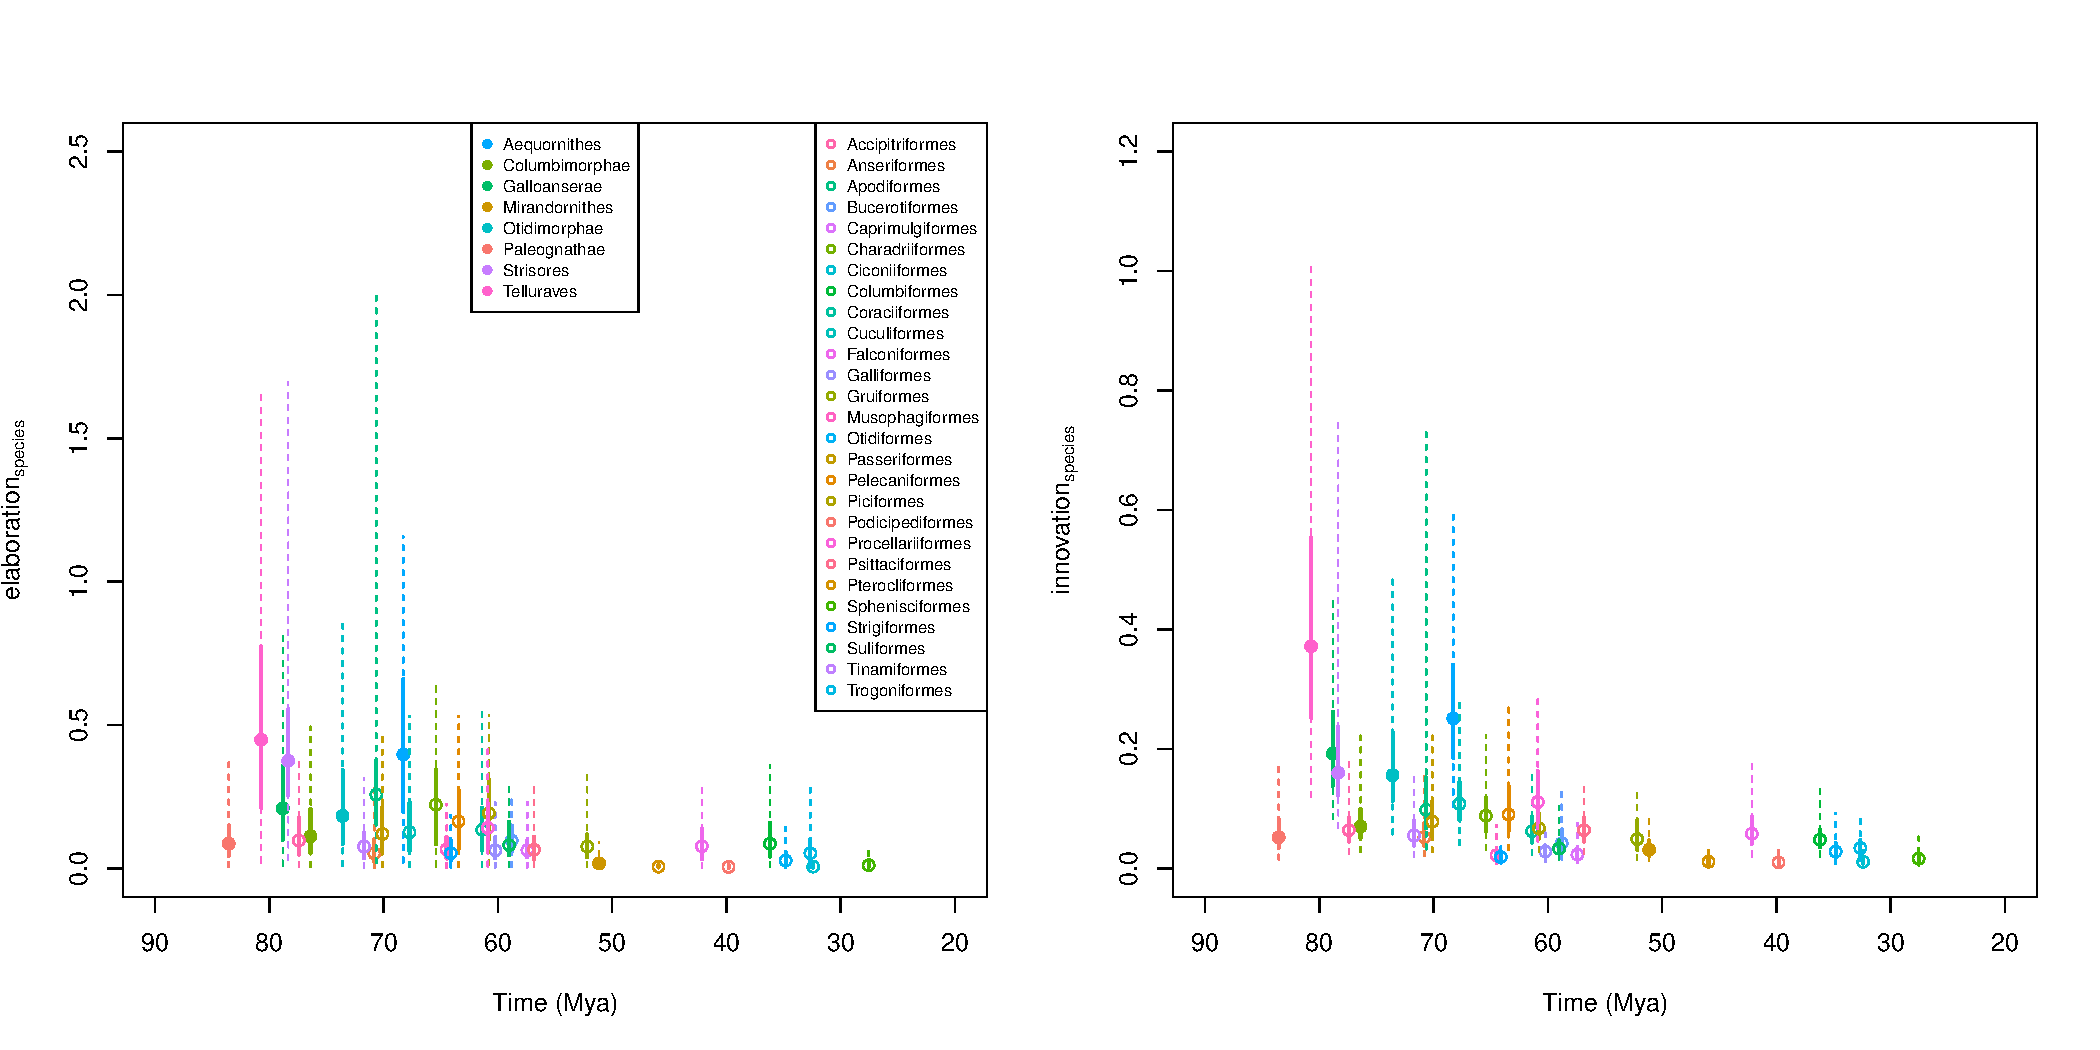
\includegraphics[width=1\textwidth]{Figures/Elaboration_and_innovation_species_through_time.pdf}
\caption{Distribution of $elaboration_{species}$ and $innovation_{species}$ for each order and super-order through time in millions of years (Mya).}
\label{Fig:figure_ei_species_through_time}
\end{figure}

\newpage

\subsection{Orientations in $elaboration_{clade}$ and $innovation_{clade}$}

\begin{figure}[H]
\centering
   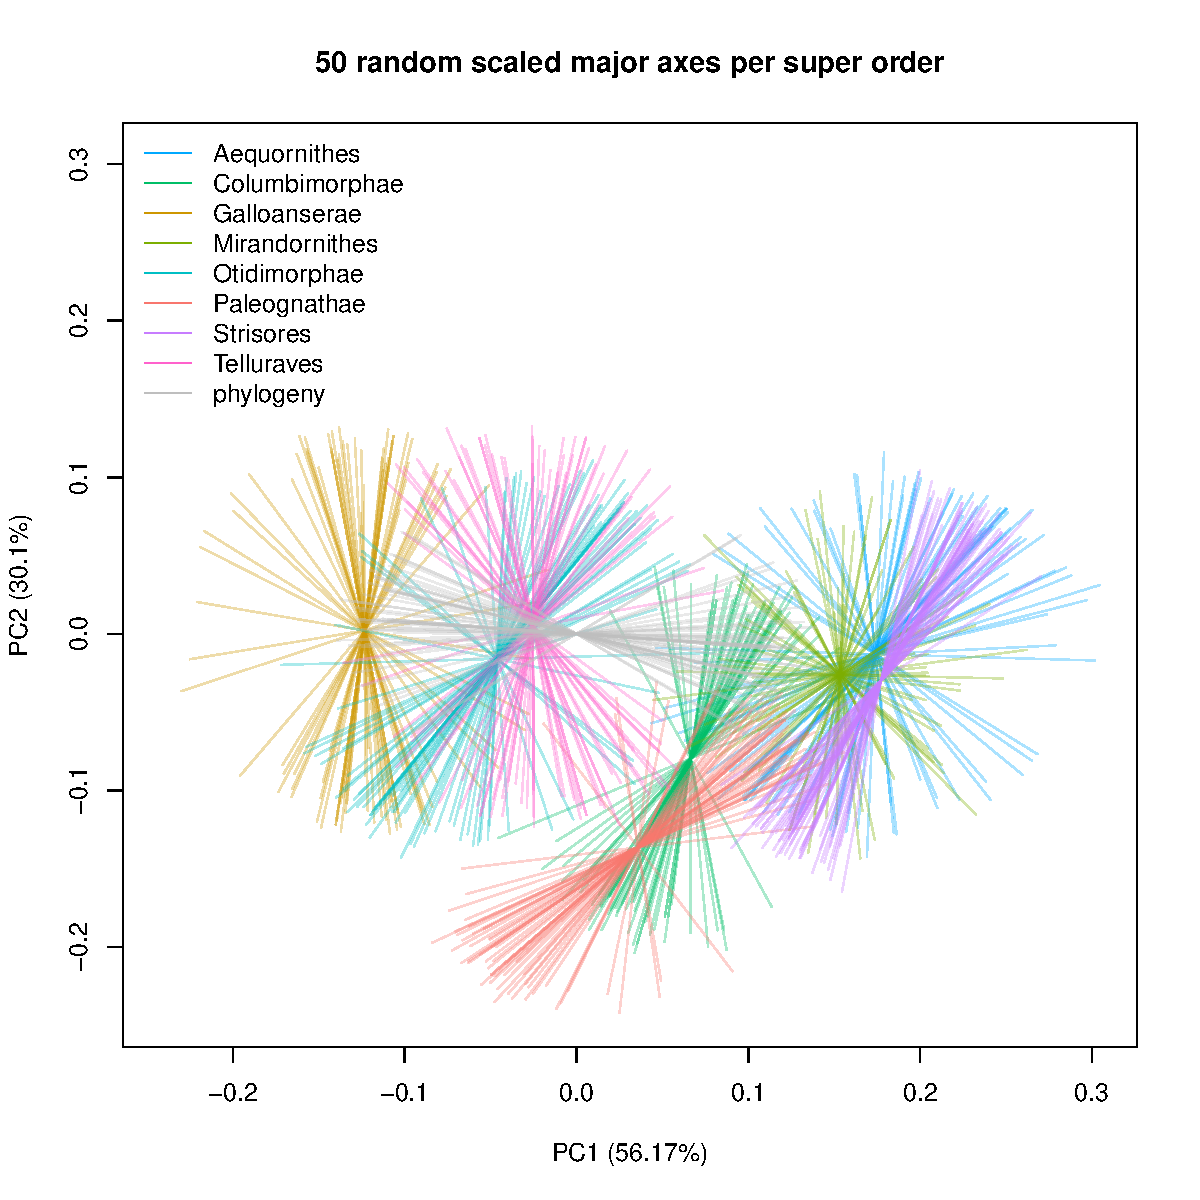
\includegraphics[width=0.5\textwidth]{Figures/50_random_axes_superorders.pdf}
\caption{Distribution of 50 random scaled major axes (scaled evolutionary rate matrices eigenvectors) for each super-order illustrating that individual phylogenetic major axes of beak variation can span many different directions and that some clades have a higher spread of directions than others.}
\label{Fig:mikado}
\end{figure}


\begin{figure}[H]
\centering
   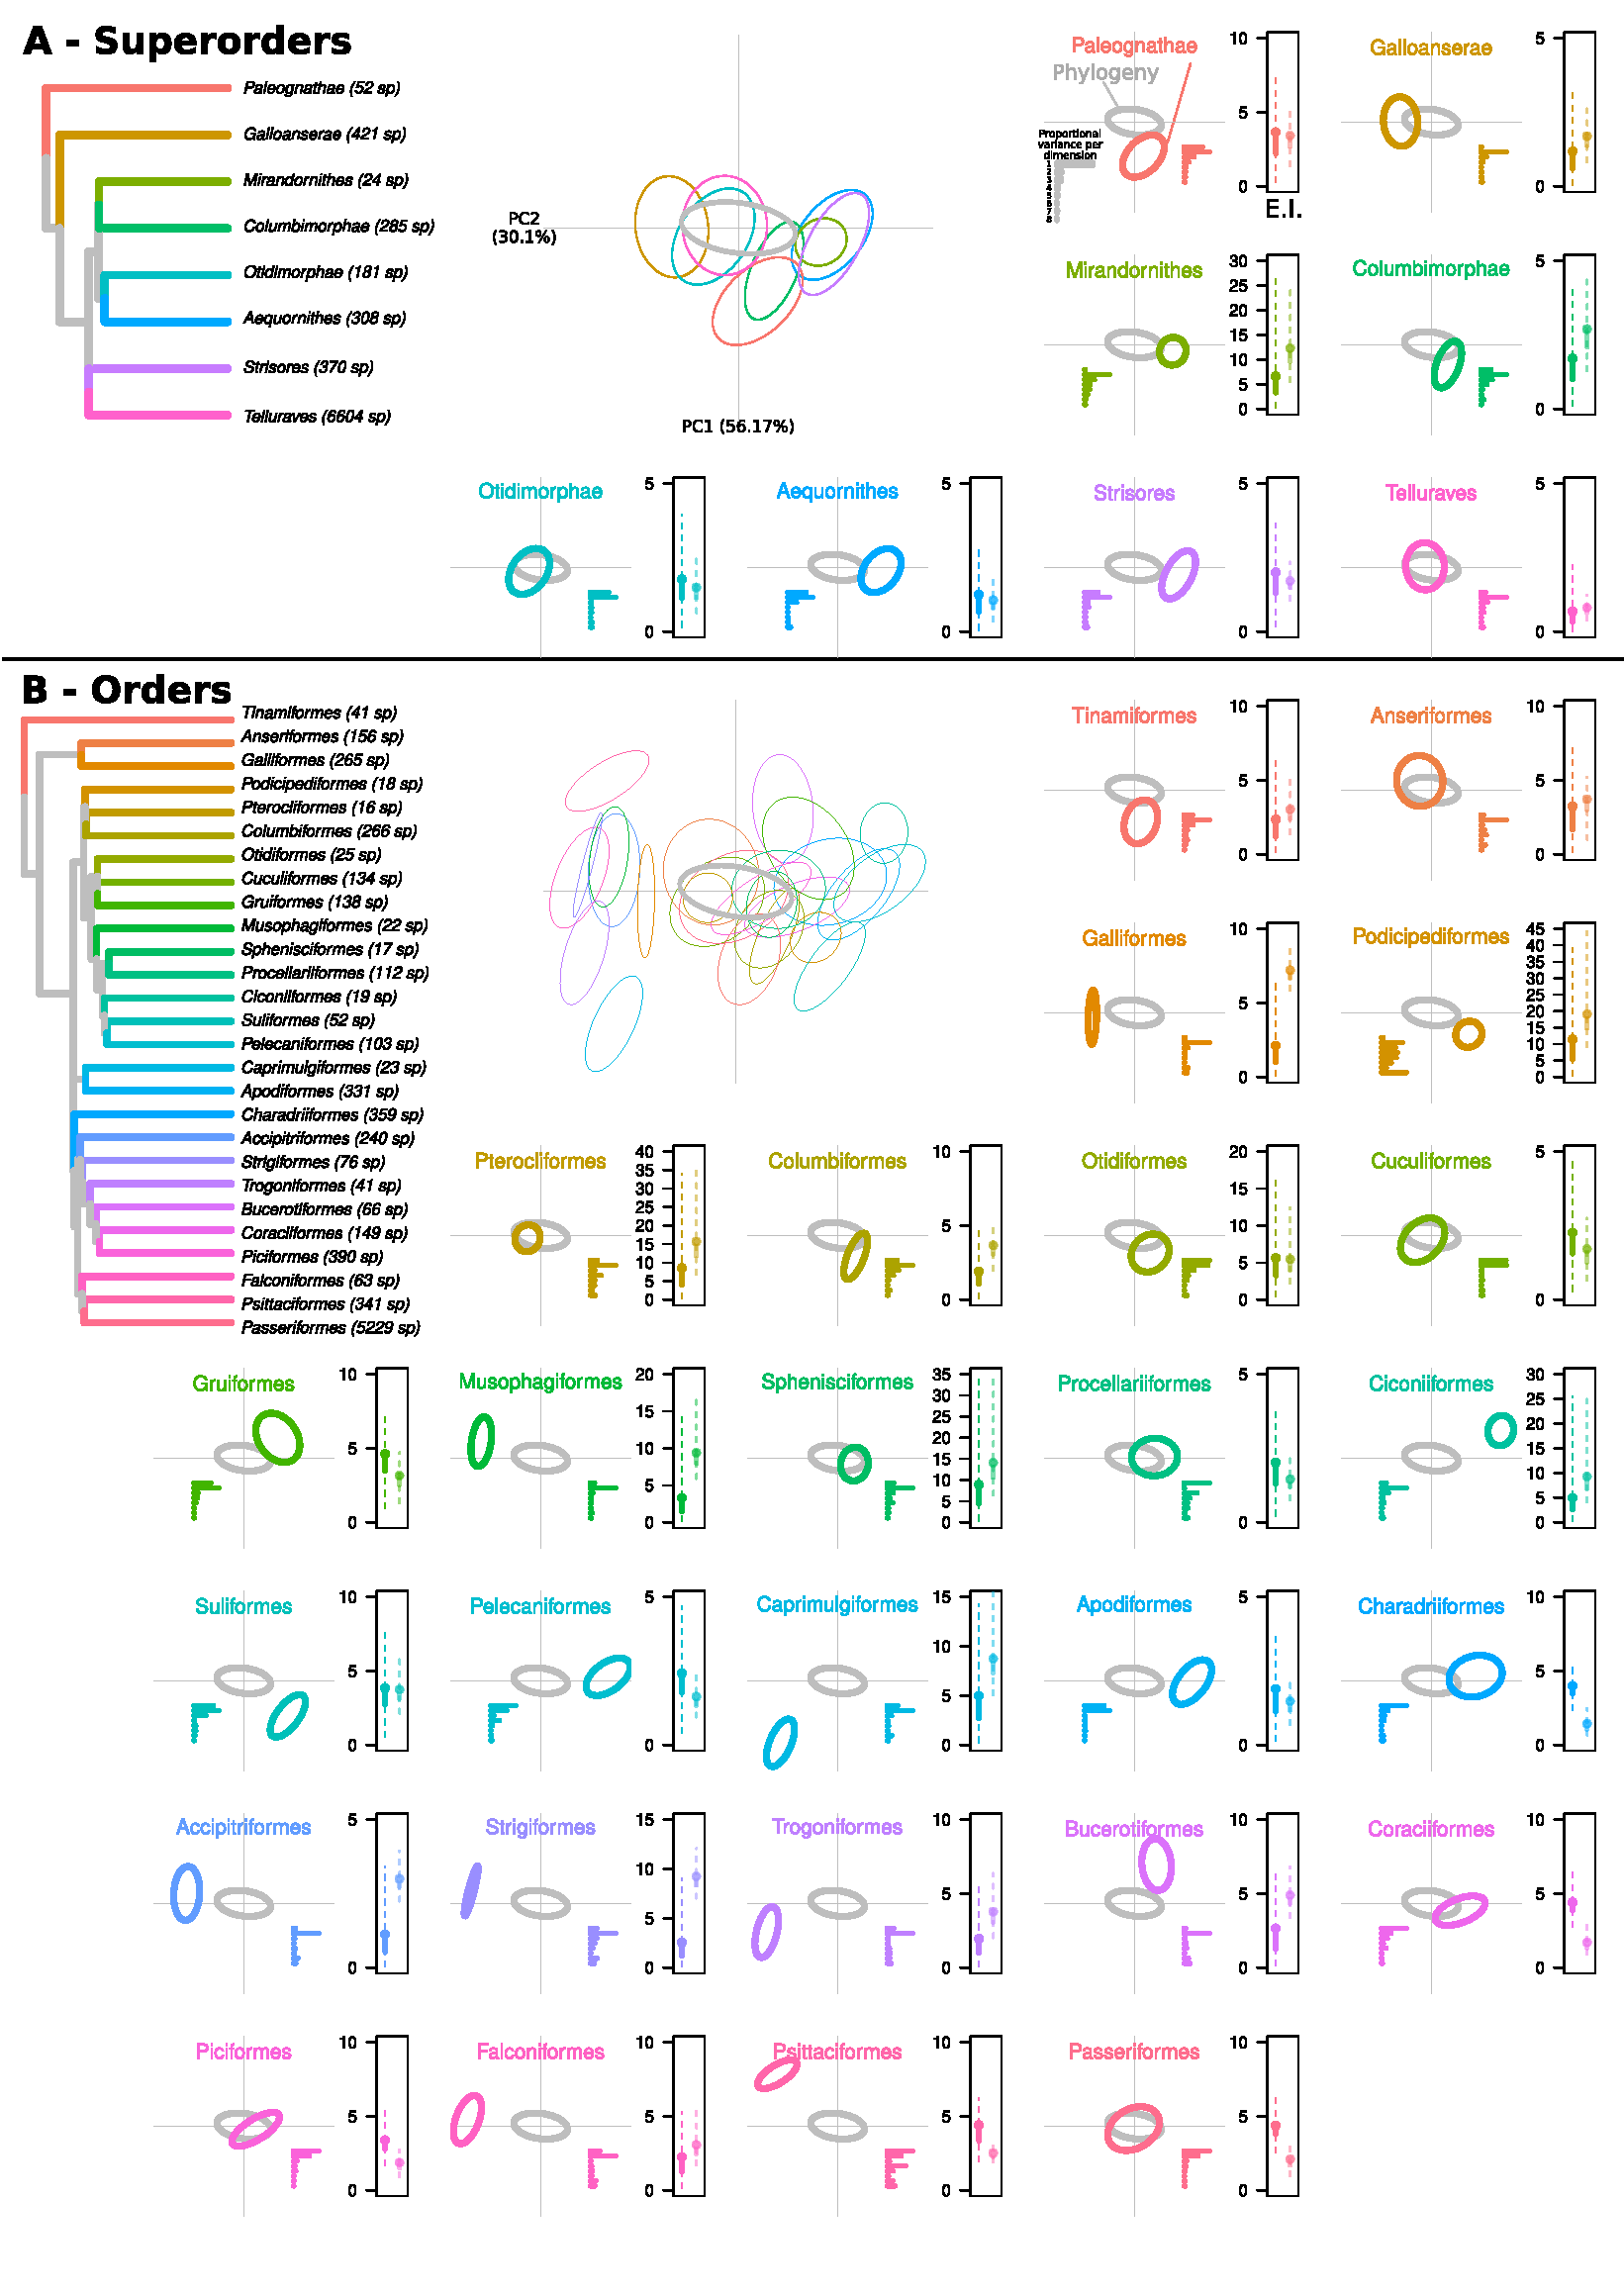
\includegraphics[width=0.8\textwidth]{Figures/ellipses_supplementary.pdf}
\caption{\scriptsize{\textbf{(A)} Ellipses representing the scaled average posterior evolutionary rate matrix from the pGLMM models for each super-order (coloured ellipses) compared to the clade-wide phylogenetic component of the models (grey ellipses).
We scaled the ellipses so the length of the phylogenetic major axis of beak variation of the clade ellipse is the same length as that of the clade-wide phylogenetic major axis ellipse (in eight dimensions).
The first inset ellipse plot shows the positions of all super-order ellipses relative to the clade-wide phylogenetic ellipse.
Subsequent inset plots show the results for each super-order. 
Inset bar plots show the proportion of variance associated with each of the eight principal component (PC) axes in shapespace.
The inset boxplots correspond to the $elaboration_{clade}$ (E) and $innovation_{clade}$ (I) scores for all 4000 posterior samples.
The dots represent the median $elaboration_{clade}$ and $innovation_{clade}$ values while the thick and dashed lines represent the 50\% and 95\% confidence intervals respectively.
These scores were calculated on the unscaled ellipses resulting in different scales of $elaboration_{clade}$ and $innovation_{clade}$ for each plot.
\textbf{(B)} Results for each order.}}
\label{Fig:ellipses_rainbow}
\end{figure}


\begin{figure}[H]
\centering
   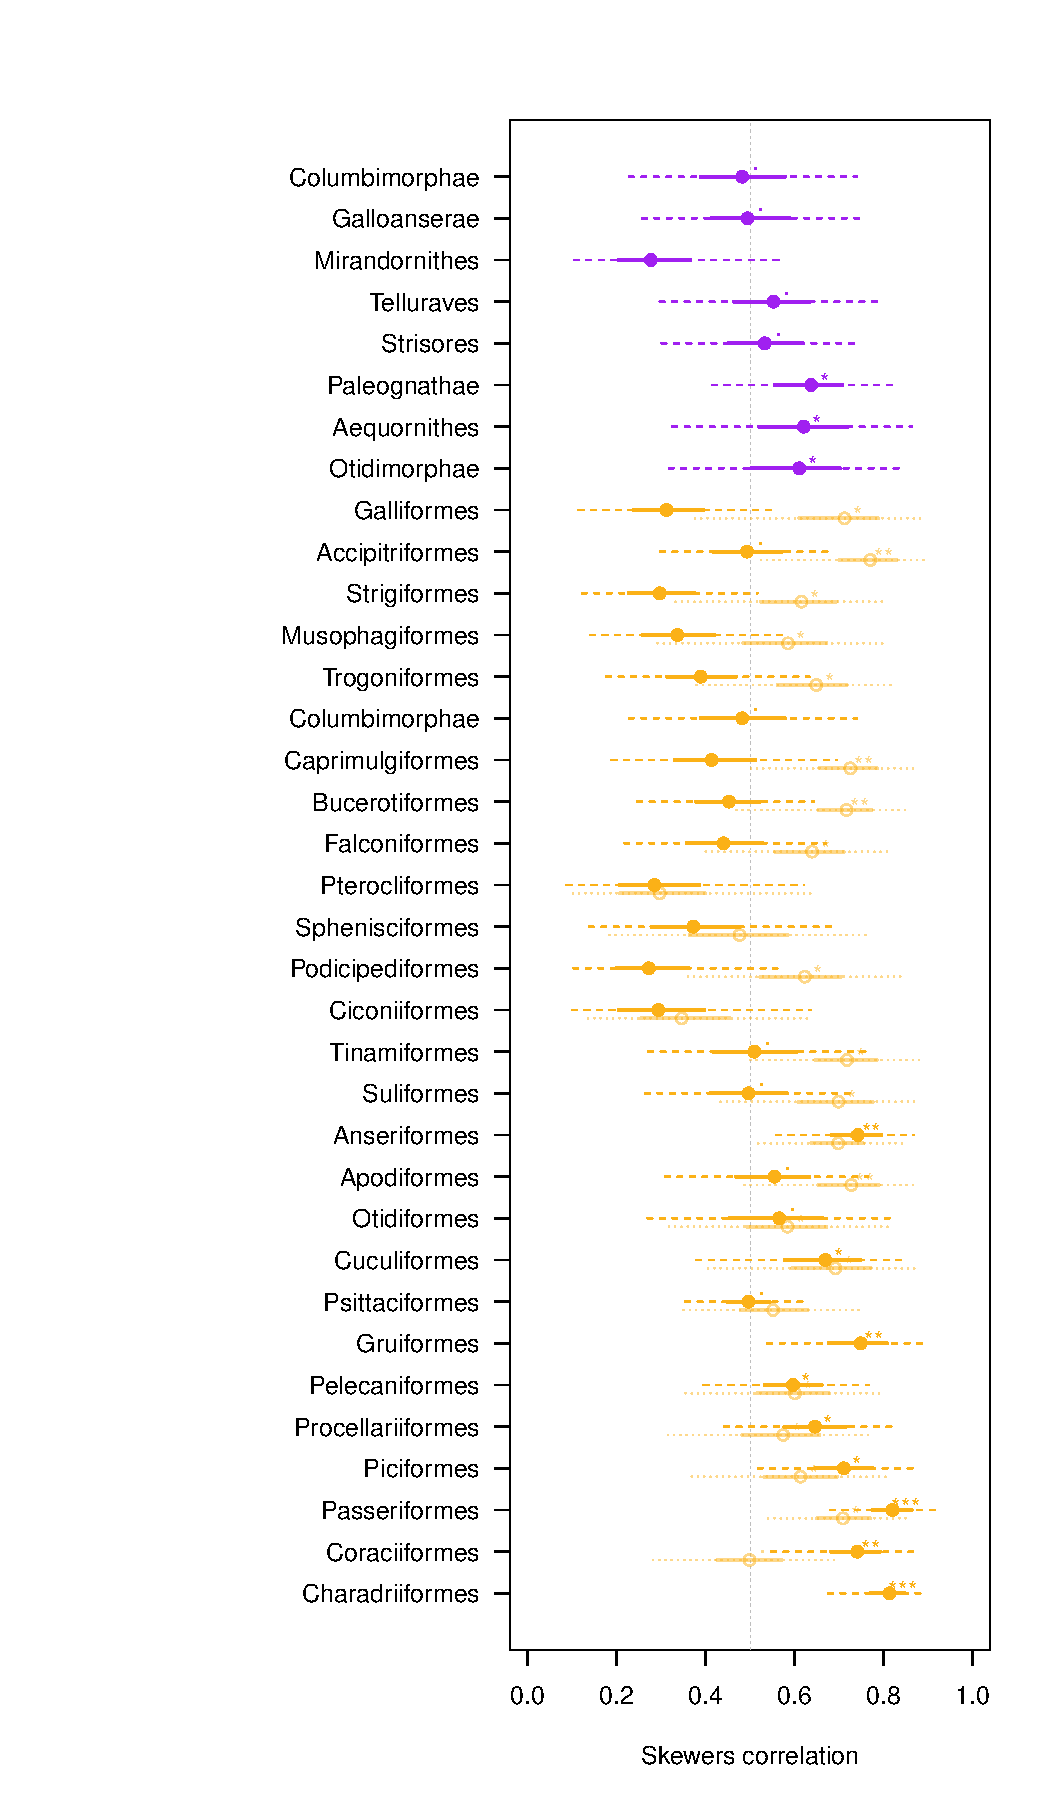
\includegraphics[width=0.5\textwidth]{Figures/random_skewers.pdf}
\caption{Random skewers test for the differences between the super-orders (in purple) and the orders (in gold) evolutionary rate matrices against the clade-wide matrices. And, in light gold, between the orders and their super-orders evolutionary rate matrices. The different line types (dashed and full) represent respectively the 95\% and the 75\% CI distribution and the dots represent the median skewer correlation estimate. The stars denote the median p-value estimate (0 ‘***’ 0.001 ‘**’ 0.01 ‘*’ 0.05 ‘.’ 0.1 ‘ ’ 1).}
\label{Fig:random_skewers}
\end{figure}

%---------------------------------------------
%
%   passeriformes results
%
%---------------------------------------------


\newpage
\clearpage
\section{Passeriformes results}

\subsection{Passeriformes $elaboration_{species}$ and $innovation_{species}$}

\begin{figure}[H]
\centering
    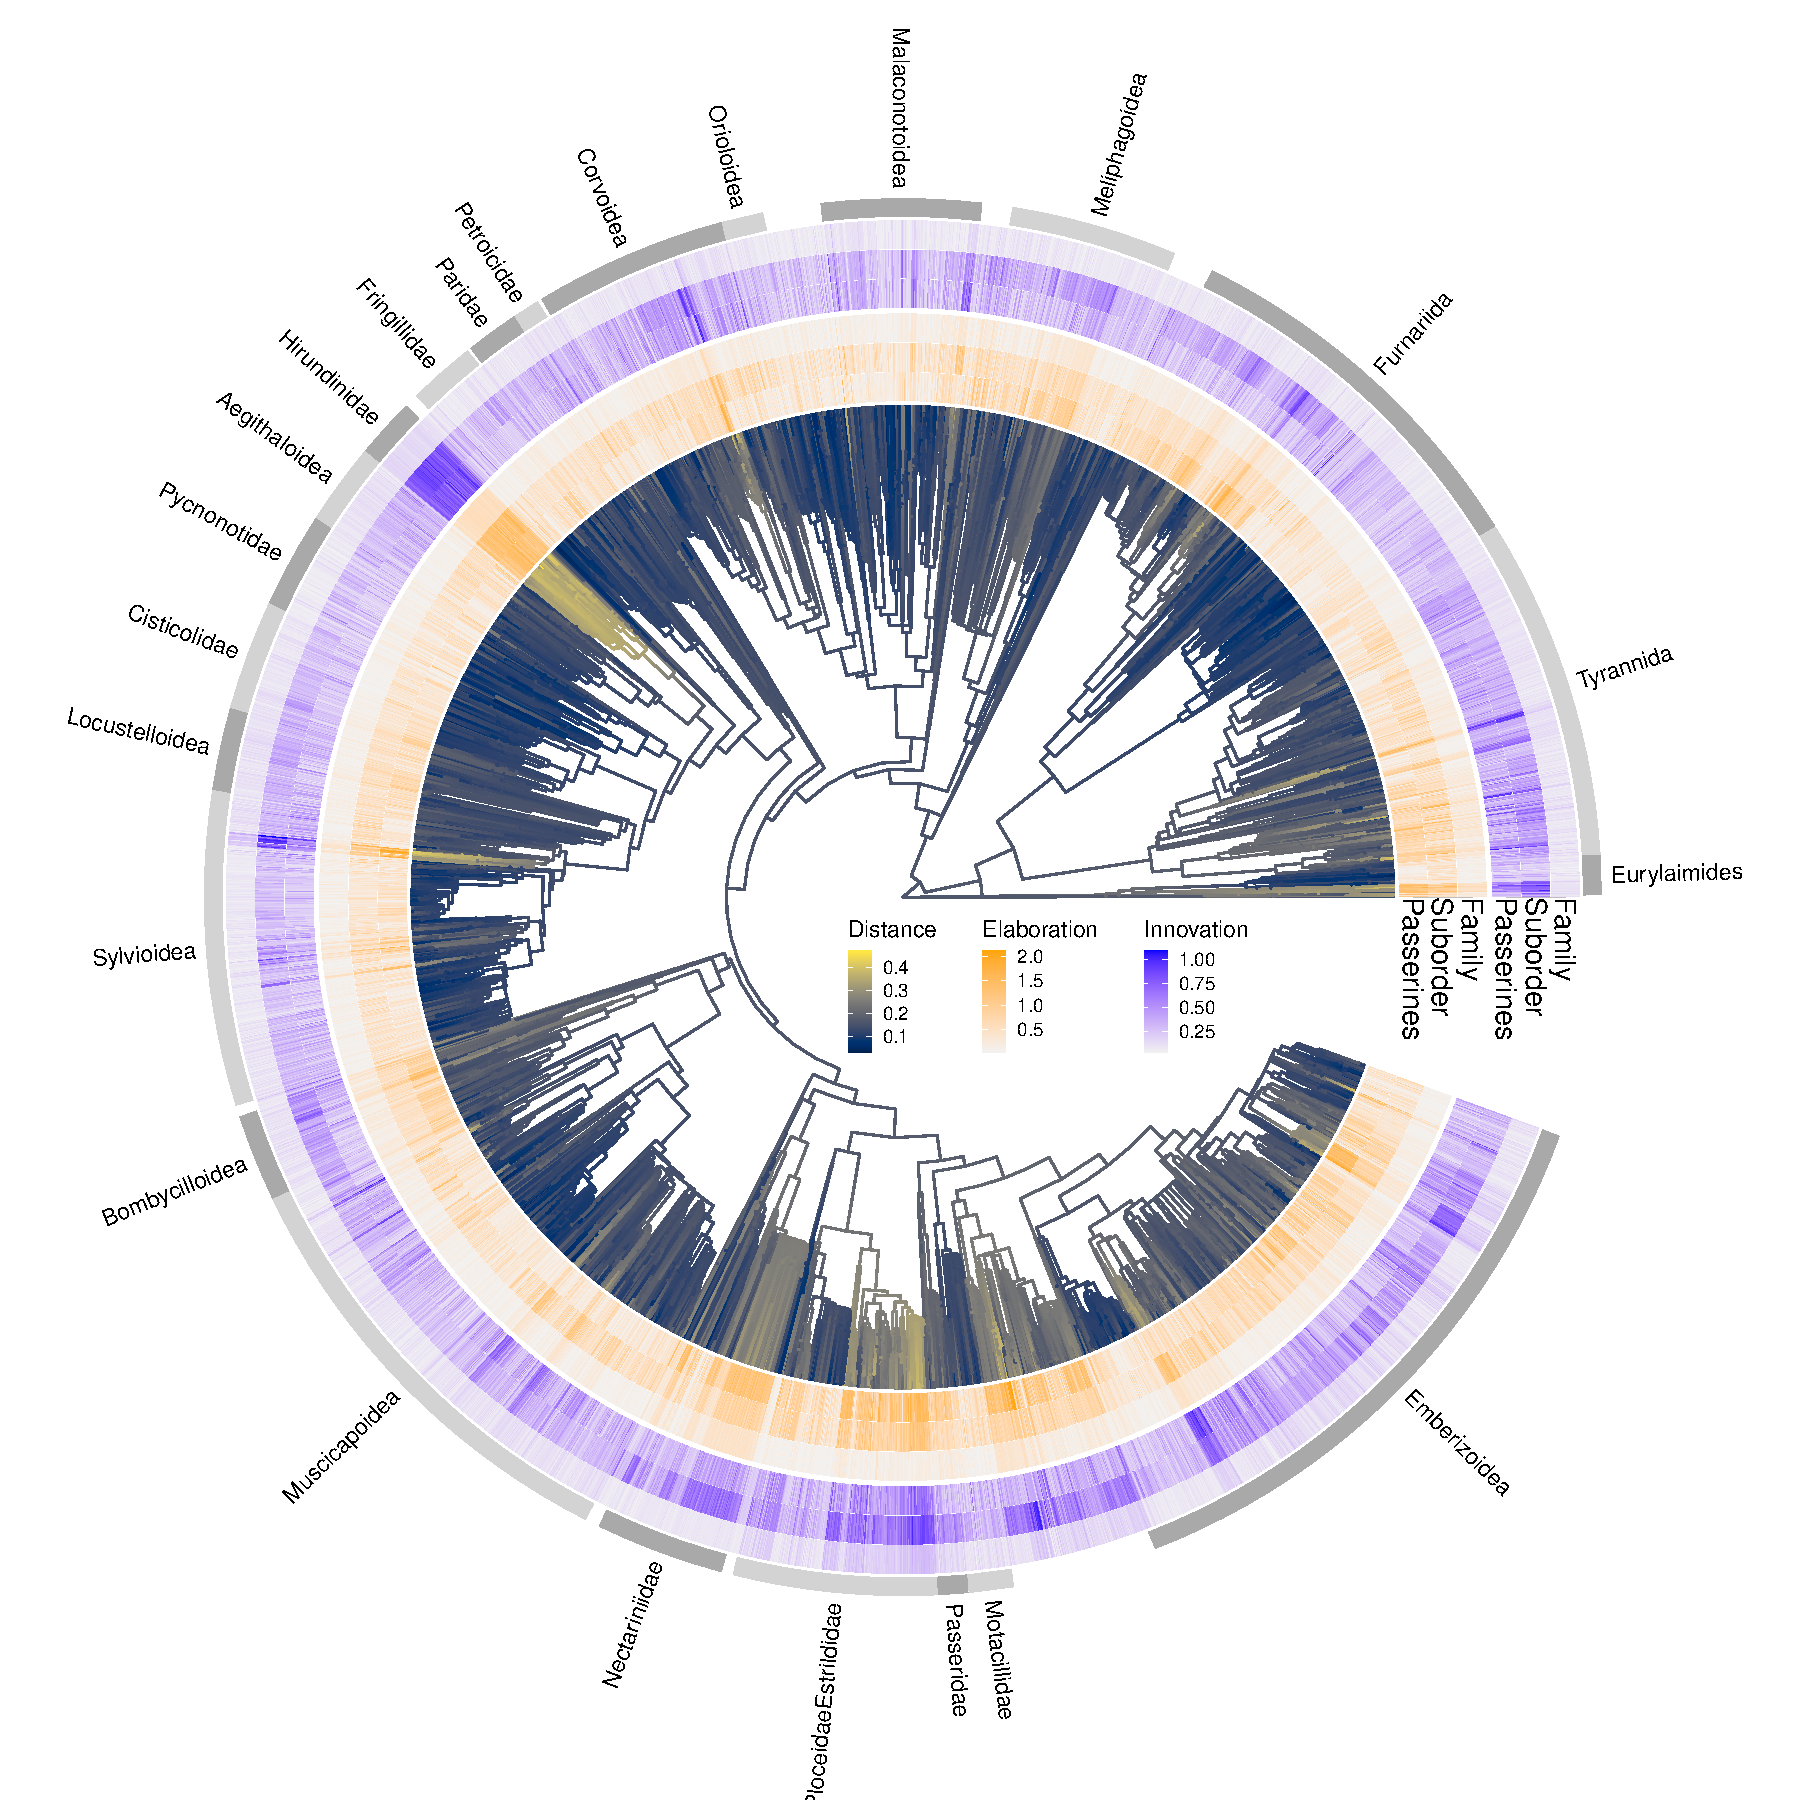
\includegraphics[width=0.9\textwidth]{Figures/InnovElabTree_passerine_supplement_revised.pdf}
\caption{Passeriformes phylogeny (n = 5229 species) showing Euclidean distance of species to the centroid of beak space (branches, cividis scale), and distributions of species beak shape $elaboration_{species}$ (inner circle, orange scale), and $innovation_{species}$ (outer circle, blue scale). Elaboration and innovation scores represent comparisons of species at the order, sub-order and family level.}
\label{fig_phylogeny_passeriformes}
\end{figure}


\newpage

\subsection{Passeriformes $elaboration_{clade}$ and $innovation_{clade}$ at the megaevolutionary scale}

\begin{figure}[H]
\centering
   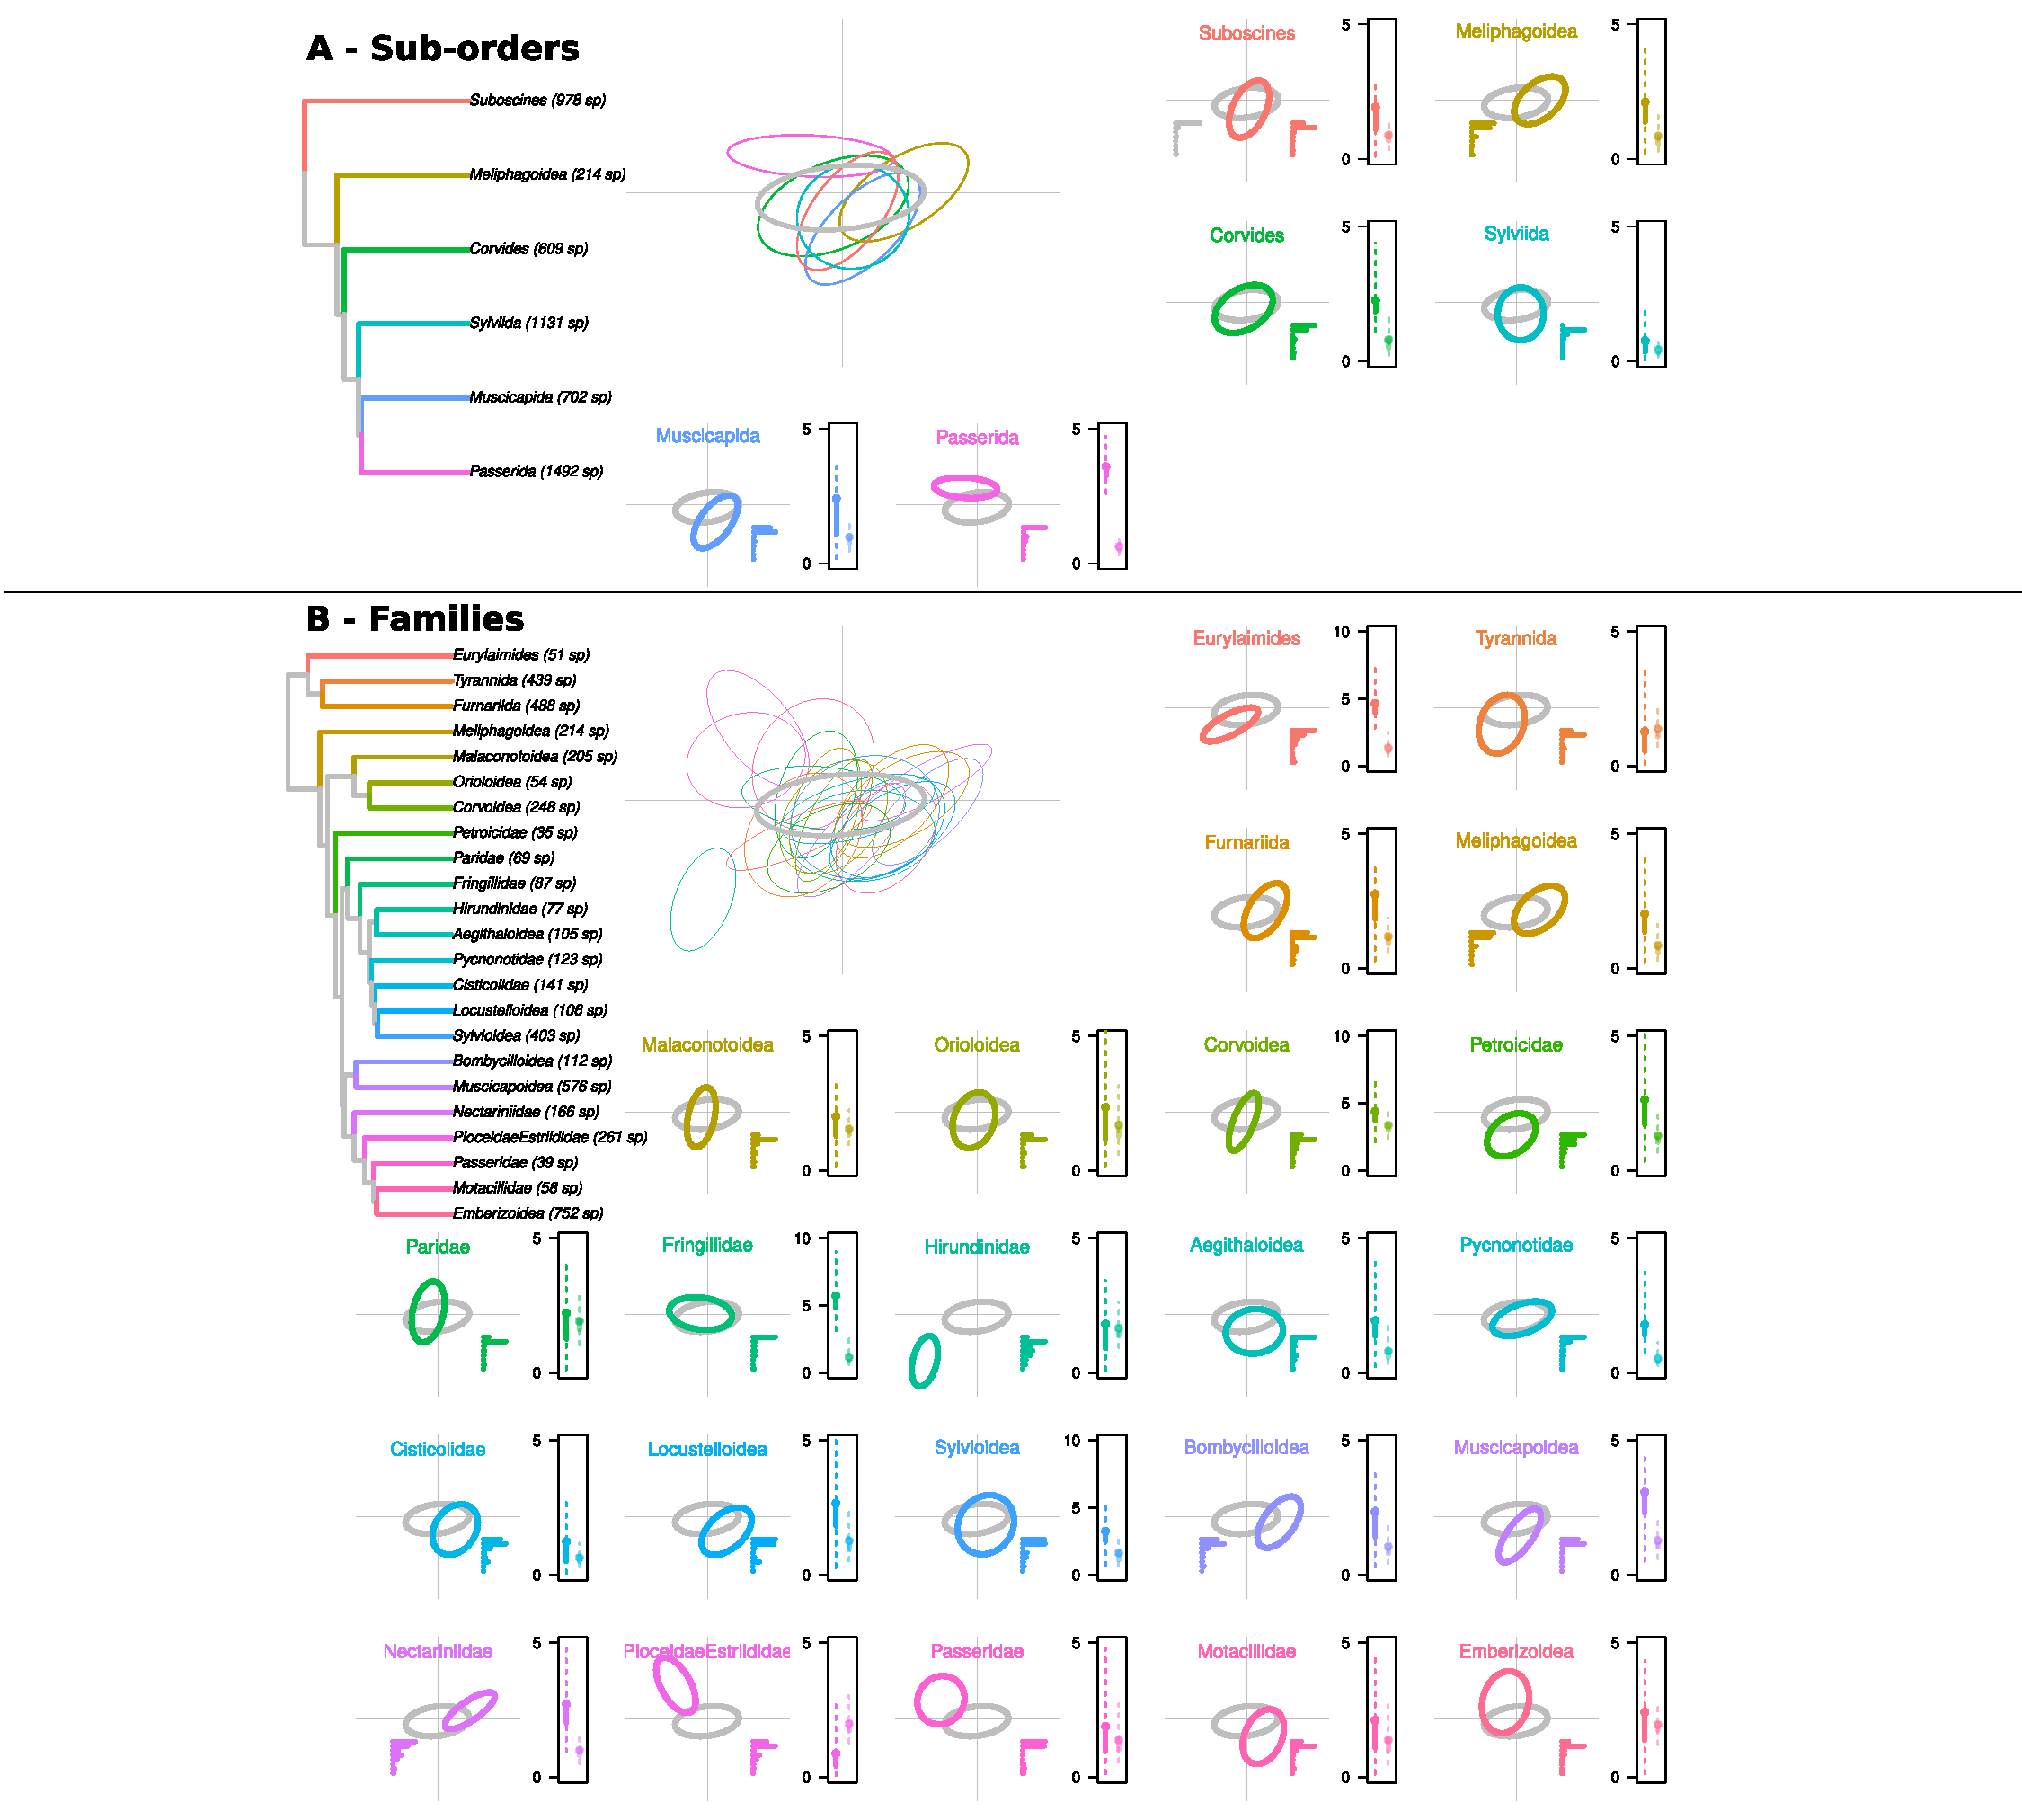
\includegraphics[width=1\textwidth]{Figures/ellipses_passeriformes.pdf}
\caption{\textbf{(A)} Ellipses representing the scaled average posterior evolutionary rate matrix from the pGLMM models for each Passeriformes sub-orders and families (coloured ellipses) compared to the Passeriformes phylogenetic component of the models (grey ellipses).
We scaled the ellipses so the length of the phylogenetic major axis of beak variation of the clade ellipse is the same length as that of the Passeriformes phylogenetic major axis ellipse (in eight dimensions).
The first inset ellipse plot shows the positions of all sub-order ellipses relative to the Passeriformes phylogenetic ellipse.
Subsequent inset plots show the results for each sub-order. 
Inset bar plots show the proportion of variance associated with each of the eight principal component (PC) axes in shapespace.
The inset boxplots correspond to the $elaboration_{clade}$ (left) and $innovation_{clade}$ (right) scores for all 4000 posterior samples.
The dots represent the median $elaboration_{clade}$ and $innovation_{clade}$ values while the thick and dashed lines represent the 50\% and 95\% confidence intervals respectively.
These scores were calculated on the unscaled ellipses resulting in different scales of $elaboration_{clade}$ and $innovation_{clade}$ for each plot.
\textbf{(B)} Results for each families.}
\label{fig_ellipses_passeriformes}
\end{figure}

\newpage

\subsection{Passeriformes orthogonality}

\begin{figure}[H]
\centering
   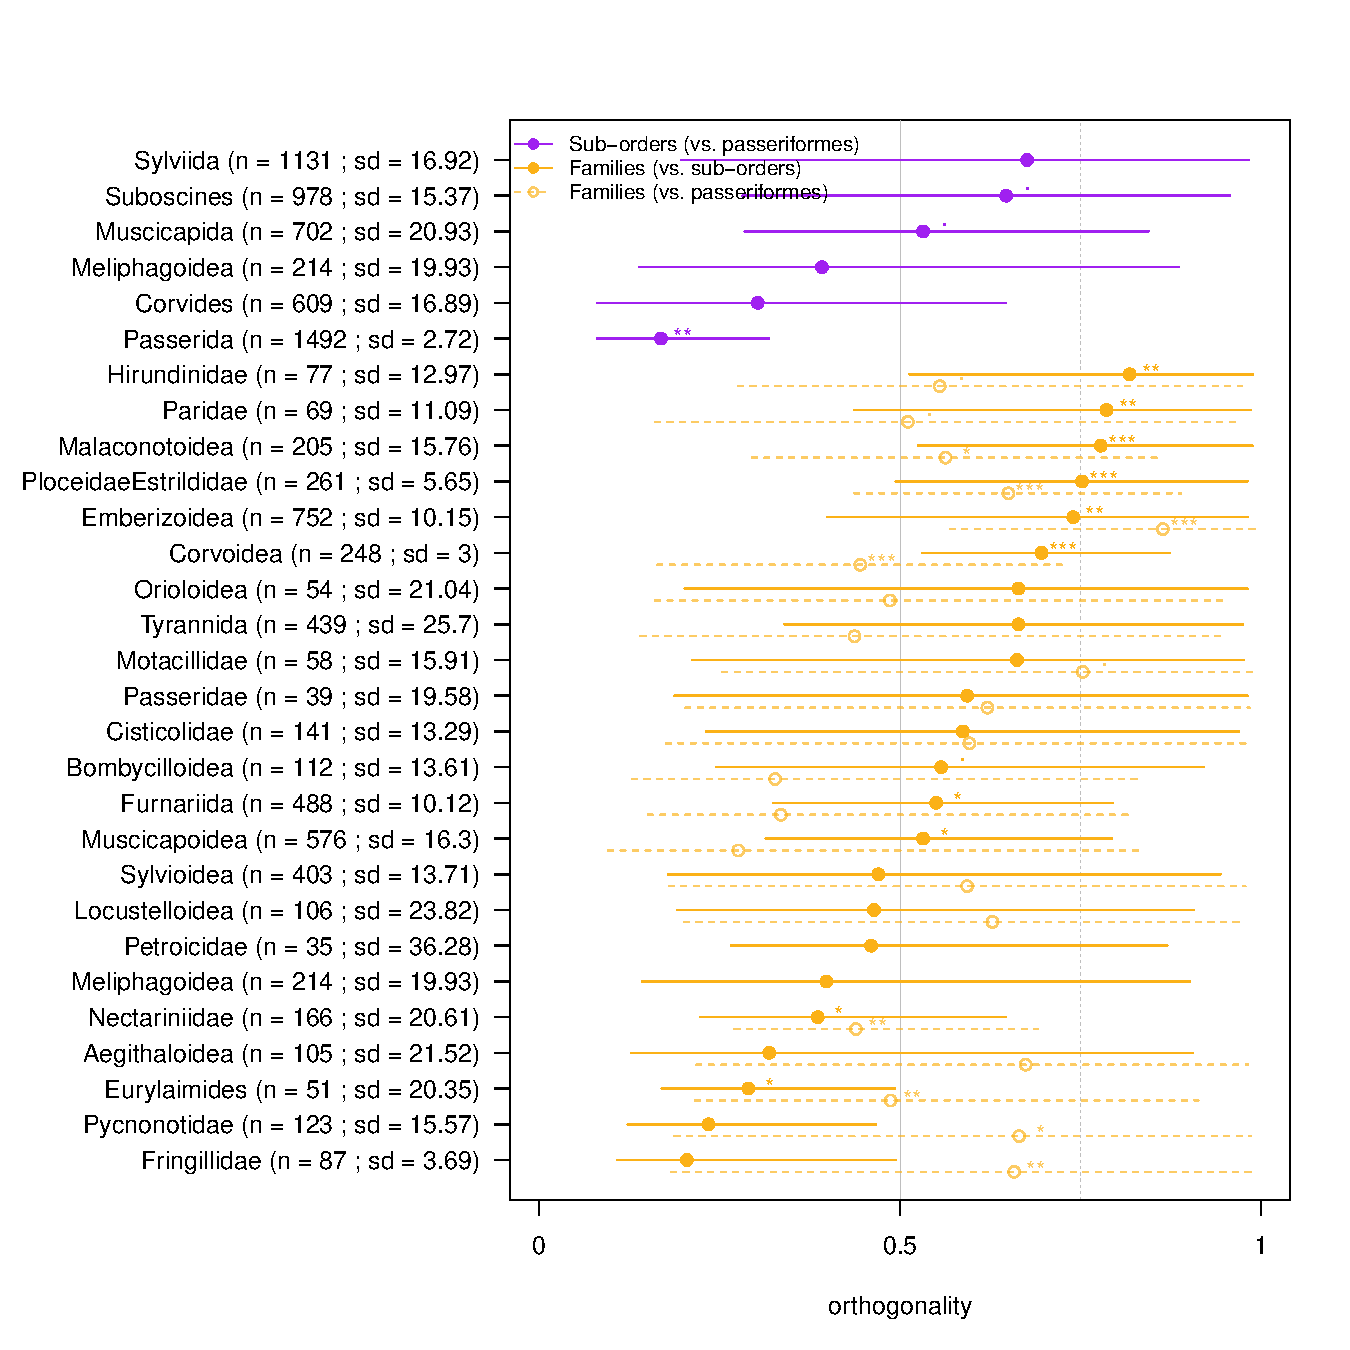
\includegraphics[width=0.9\textwidth]{Figures/orthogonality_results_passeriformes.pdf}
\caption{Amount of orthogonality of each Passeriformes sub-order's and family's phylogenetic major axis of beak variation compared to their parent or parent's parent clade.
The amount of orthogonality is represented on the horizontal axis and scales from 0 (modulo of $0^\circ$) to 1 (modulo of $90^\circ$) with the background gray and dashed gray lines representing, respectively, an orthogonality of 0.5 (modulo of $45^\circ$) and 0.75 (modulo of $67.5^\circ$).
Dots represent the median orthogonality of each clade and the lines their 95\% confidence intervals (CI).
We also indicate the number of species (n) and the standard deviation (sd) of the orientation of their phylogenetic major axis of beak variation over the 4000 variance-covariance posteriors (sd; expressed in degrees).
For each clade we also measured the posterior probability of each clade's orientation being different from their parent's clade or the class-wide phylogenetic major axis of beak variation relative to their sample size and sd.
The stars represent the posterior probability of the clade's orientation being different from the comparison clade (*** = pp $> 0.99$; ** = pp $>0.95$; * = pp $> 0.9$; . = pp $> 0.8$).}
\label{fig_orthogonality_passeriformes}
\end{figure}

%---------------------------------------------
%
%   maths
%
%---------------------------------------------

\newpage

\section{Detailed projection and rejection operations for measuring elaboration and innovation}
\label{supp_projection}

The following section contains the detailed definition and procedure of how we measured elaboration and innovation.

We can define the major axis from the variance-covariance matrices and then project and reject each element of interest in the space onto this axis.
The following steps are generalised to $n$ dimensions and detailed below (as well as the algorithm used in \texttt{dispRity} [64]%\cite{dispRity}
to perform the transformations):

\subsection{Defining the major axis}

For $O_{n}$, the unit hypersphere matrix of $n$ dimensions and a radius composed of the two identity matrices $I_{n}$ and $-I_{n}$ so that: 

\begin{equation}
O_{n} = 
    \begin{pmatrix}
        1 & 0 & \cdots & 0 \\
        0 & 1 & \cdots & 0 \\
        \vdots  & \vdots  & \ddots & \vdots  \\
        0 & 0 & \cdots & 1 \\
        -1 & 0 & \cdots & 0 \\
        0 & -1 & \cdots & 0 \\
        \vdots  & \vdots  & \ddots & \vdots  \\
        0 & 0 & \cdots & -1 \\
    \end{pmatrix}
\end{equation}

In other words, $O_{n}$ is the matrix representing the hypersphere of $n$ dimensions and of radius $1$ that fits in the centre of the trait-space;

And $O'_{n}$ is the scaled matrix hypersphere to the 95\% confidence interval size using the $\chi^2$ distribution:

$$O'_{n} = O_{n} \sqrt{\chi^2(0.95)}$$

Then, for the variance-covariance matrix $VCV_{n}$ of $n$ dimensions obtained from the posterior distribution of the \texttt{mcmcmcglmmmm}:

\begin{equation}
VCV_{n} = 
    \begin{pmatrix}
        \sigma(a) & \sigma(a,b) & \cdots & \sigma(a,n) \\
        \sigma(a,b) & \sigma(b) & \cdots & \sigma(b,n) \\
        \vdots  & \vdots  & \ddots & \vdots  \\
        \sigma(n,a) & \sigma(n,b) & \cdots & \sigma(n) \\
    \end{pmatrix}
\end{equation}

and the eigenvectors \textbf{v} and the eigenvalues $\lambda$ satisfying the following eigen decomposition:

$$VCV_{n} \textbf{v} = \lambda \textbf{v}$$

We can get $M_{n}$, the matrix containing all the edge coordinates of the 0.95 CI hypersphere from $VCV_{n}$ using the transposition of the cross product between the eigenvectors \textbf{v} and the product of the scaled 0.95 CI unit sphere $O'_{n}$ and the eigenvalues $\lambda$:

$$M_{n} = [(O'_{n}\sqrt{\lambda}) \times v]^{\text{T}}$$

Finally, we can centre the matrix $M_{n}$ on the estimated solution of each GLMM (\texttt{model\$Sol}, in \texttt{MCMCglmm} [48]% \cite{MCMCglmm}
) corresponding to the estimation of the position of the variance-covariance matrix in the trait-space.
$M_{n}$ then contains all the major axes of the 0.95 hyper-ellipse fitting the variance-covariance matrix.
We can then define the first row of the matrix, $M_{1,n}$, as the major axis, the second row, $M_{2,n}$, as the second major axis (the minor axis in a 2D ellipse), etc.

The detailed procedure was adapted from \href{https://stackoverflow.com/questions/40300217/obtain-vertices-of-the-ellipse-on-an-ellipse-covariance-plot-created-by-care/40316331#40316331}{Zheyuan Li's} post on Stack Overflow and implemented in \texttt{dispRity::axis.covar}.

The use of the scaled 95\% confidence interval hyper-sphere matrix $O'_{n}$ allows both (1) to standardise the resulting $M_{n}$ (the scaled version of $VCV_{n}$) so that the unit vector of the resulting space corresponds to the 95\% CI on every dimension (for any dimension $i$ in the matrix $M_{i,n}$, any vector with a norm smaller or greater than 1 is respectively inside or outside the 95\% CI boundary).
And (2) greatly speed up the calculations of projection and rejection in an algorithm (see below) since the hypersphere $O'_{n}$ can be calculated only once for any number of matrix and the projection of rejection values are directly columns in the output transformed matrix (after the projection procedure, see below).
This greatly reduces RAM and CPU usage and scaling for very large number of matrices.

\subsection{Measuring projection and rejection}

Once we have defined a major axis, we can project any elements in the trait-space onto that axis.
Specifically, for any elements in the trait-space, we can define it as the vector $\vec{a}$ with one set of coordinates in $n$ dimensions:

\begin{equation}
    \vec{a} = 
    \begin{bmatrix}
    x \\
    y \\
    \cdots \\
    n \\
    \end{bmatrix}
\end{equation}

And for any major axis that we can define as a vector $\vec{b}$ as a set of pairs of coordinates in $n$ dimensions:

\begin{equation}
    \vec{b} = 
    \begin{bmatrix}
    x_{1} & x_{2} \\
    y_{1} & y_{2} \\
    \cdots & \cdots \\
    n_{1} & n_{2} \\
    \end{bmatrix}
\end{equation}

We can then calculate $\vec{a_{1}}$, the orthogonal projection of $\vec{a}$ onto $\vec{b}$ using:

\begin{equation}
    \vec{a_{1}} = \frac{\vec{a} \cdot \vec{b}}{\|\vec{b}\|}
\end{equation}


\begin{equation}
    \vec{a_{1}} = \frac{\vec{a} \cdot \vec{b}}{\|\sqrt{\vec{b} \cdot \vec{b}}\|}
\end{equation}


With $\|\vec{b}\| = \sqrt{\vec{b} \cdot \vec{b}}$ being the norm of $\vec{b}$.
And $\vec{a_{2}}$, the rejection of $\vec{a}$ onto $\vec{b}$:

\begin{equation}
    \vec{a_{2}} = \vec{a} - \vec{a_{1}}
\end{equation}

\subsubsection{Generalisation of projection onto any vector in a set space}

Using this, we can generalise the procedure so as to calculate the projection and rejection for any element within a trait-space $TS_{m,n}$:

\begin{equation}
    TS_{m,n} = 
    \begin{bmatrix}
    x_{1} & x_{2} & \cdots & x_{m} \\
    y_{1} & y_{2} & \cdots & y_{m} \\
    \vdots  & \vdots  & \ddots & \vdots \\
    n_{1} & n_{2} & \cdots & n_{m} \\
    \end{bmatrix}
\end{equation}

And any major axis defined as a vector $\vec{B}$:

\begin{equation}
    B = 
    \begin{bmatrix}
    x_{1} & x_{2}\\
    y_{1} & y_{2}\\
    \vdots  & \vdots  \\
    n_{1} & n_{2} \\
    \end{bmatrix}
\end{equation}


By using the linear transformation $f_{\vec{B}}$ of the trait-space $TS$ moving $\vec{B}$ onto $TS$'s first axis unit vector $\vec{\hat{\imath}}$:

$$f_{\vec{B}}(TS) = \left( \frac{TS - [Bx_{1}, By_{1}, \cdots, Bn_{1}]^{\text{T}}}{\|\vec{B}\|} \right) \cdot R_{\vec{B}}$$

With $R_{\vec{B}}$ being the rotation matrix of the vector $\vec{B}$ onto $\vec{\hat{\imath}}$:

\begin{equation}
R_{\vec{B}} = I_{\vec{B}} - \vec{B}\vec{B}^\text{T} - \vec{\hat{\imath}}\vec{\hat{\imath}}^\text{T} + [\vec{B} \vec{\hat{\imath}}]
    \begin{bmatrix}
        cos(\theta) & -sin(\theta)\\
        sin(\theta) & cos(\theta)\\
    \end{bmatrix} [\vec{B} \vec{\hat{\imath}}]^\text{T}
\end{equation}

Where $\theta$ is:

\begin{equation}
    \theta = acos \left(\frac{\vec{B} \cdot \vec{\hat{\imath}}}{\|\vec{B}\| \cdot \|\vec{\hat{\imath}}\|} \right)
\end{equation}

Or $\theta = acos (B_x)$ since both $\|\vec{B}\|$ and $\|\vec{\hat{\imath}}\|$ are equal to 1 and $\|\vec{\hat{\imath}}\|$ is the unit vector on the first axis.

\subsection{Algorithm for calculating the projection/rejection of any element in a defined space}

In practice we followed \href{https://math.stackexchange.com/questions/598750/finding-the-rotation-matrix-in-n-dimensions}{this procedure} and applied a modification of \href{https://stackoverflow.com/questions/42520301/find-rotation-matrix-of-one-vector-to-another-using-r/42542385#42542385}{this implementation} (see [65]% \cite{aguilera2004}
 for the formal generalisation of this algorithm in $n$ dimensions) using the following algorithm implemented in \texttt{dispRity::projections}:

\begin{enumerate}
 \item In the trait-space, define $\vec{B}$ as the base vector (typically $\vec{B}$ is defined as the pair of coordinates from the major axis described above).
 \item Centre the trait-space on the origin of $\vec{B}$ so that the first set of coordinates of $\vec{B}$ are 0.
 \item Scale the trait-space to the norm of $\vec{B}$ so that the norm of $\vec{B}$ is now 1.
 \item Rotate the trait-space using the rotation matrix $R_{\vec{B}}$ to satisfy the linear transformation $\vec{B} \rightarrow \vec{\hat{\imath}}$ (with $\vec{\hat{\imath}}$ being the first unit vector of the trait-space - typically the x axis unit vector). 
 \item Project/reject every element in the trait-space on $\vec{B}$ (that is now $\vec{\hat{\imath}}$). In practice, the first coordinate (x) of each element is now its projection onto $\vec{B}$.
\end{enumerate}


\subsection{Definition of species and clade innovation and elaboration}

From the definitions above, we can define $\text{elaboration}_{\text{species}}$ and $\text{innovation}_{\text{species}}$, the elaboration and innovation at the macroevolutionary (species level) and $\text{elaboration}_{\text{clade}}$ and $\text{innovation}_{\text{clade}}$, the elaboration and innovation at the megaevolutionary level (clade).

For any species with coordinates $\vec{species}$ in a $n$ dimensional space, we can estimate $VCV_{clade}$, the variance-covariance matrices representing the clade that contains $\vec{species}$.
We can then calculate the eigen vector and eigenvalues from these matrices as: 

$\textbf{v}_{clade}$ defined as:

\begin{equation}
VCV_{clade} \textbf{v}_{clade} = \lambda_{clade} \textbf{v}_{clade}
\end{equation}

In practice, these are solved using a eigen decomposition in \texttt{R} \texttt{base::eigen}.

We can then define the followings for any species $x$:

\begin{equation}
\text{elaboration}_{\text{species}_{x}} = \|\frac{\vec{species}_{x} \cdot \textbf{v}_{clade}} {\sqrt{\textbf{v}_{clade} \cdot \textbf{v}_{clade}}}\|
\end{equation}

With $\vec{species}_{x}$ being the vector in $n$ dimensional space for species $x$. And $\textbf{v}_{clade}$ being the eigen vector of a specific clade (e.g. $\textbf{v}_{clade_{c}}$)

\begin{equation}
\text{innovation}_{\text{species}_{x}} = \| \vec{species}_{x} - \text{elaboration}_{\text{species}_{x}} \|
\end{equation}

And the followings for any clade $c$ (withing a parent clade $c-1$):

\begin{equation}
\text{elaboration}_{\text{clade}_{c}} = \| \frac{\textbf{v}_{clade_{c}} \cdot \textbf{v}_{clade_{c-1}}} {\sqrt{\textbf{v}_{clade_{c-1}} \cdot \textbf{v}_{clade_{c-1}}}}\|
\end{equation}

\begin{equation}
\text{innovation}_{\text{clade}_{c}} = \| \textbf{v}_{clade_{c}} - \text{elaboration}_{\text{clade}_{c}} \|
\end{equation}


\subsection{Relation between elaboration and innovation and metrics in micro/macro-evolution}

\subsubsection{Relative eigenvalues dispersion}

[44, 66] %\cite{vanvalen1974,watanabe2022}
propose to describe a variance-covariance matrix in terms of its eigen dispersion $V_{rel}$ as:

\begin{equation}
V_{rel} = \frac{\sum_{i}^{n}(\lambda_{i} - \sum{\frac{\lambda_{i}}{n}})^2}{n(n-1)\sum{\frac{\lambda_{i}}{n}}^2}
\end{equation}

Which is the dispersion of eigenvalues (squared difference between each eigen value and the average eigen value) where $\lambda_{i}$ are each individual eigen values and $n$ is the number of dimensions considered.

Using this definition and the definitions above of $\text{elaboration}_{\text{clade}_{c}}$ and $\text{innovation}_{\text{clade}_{c}}$ we can calculate the and plot the relation between elaboration and innovation and their relative eigen dispersion:

\begin{figure}[H]
\centering
   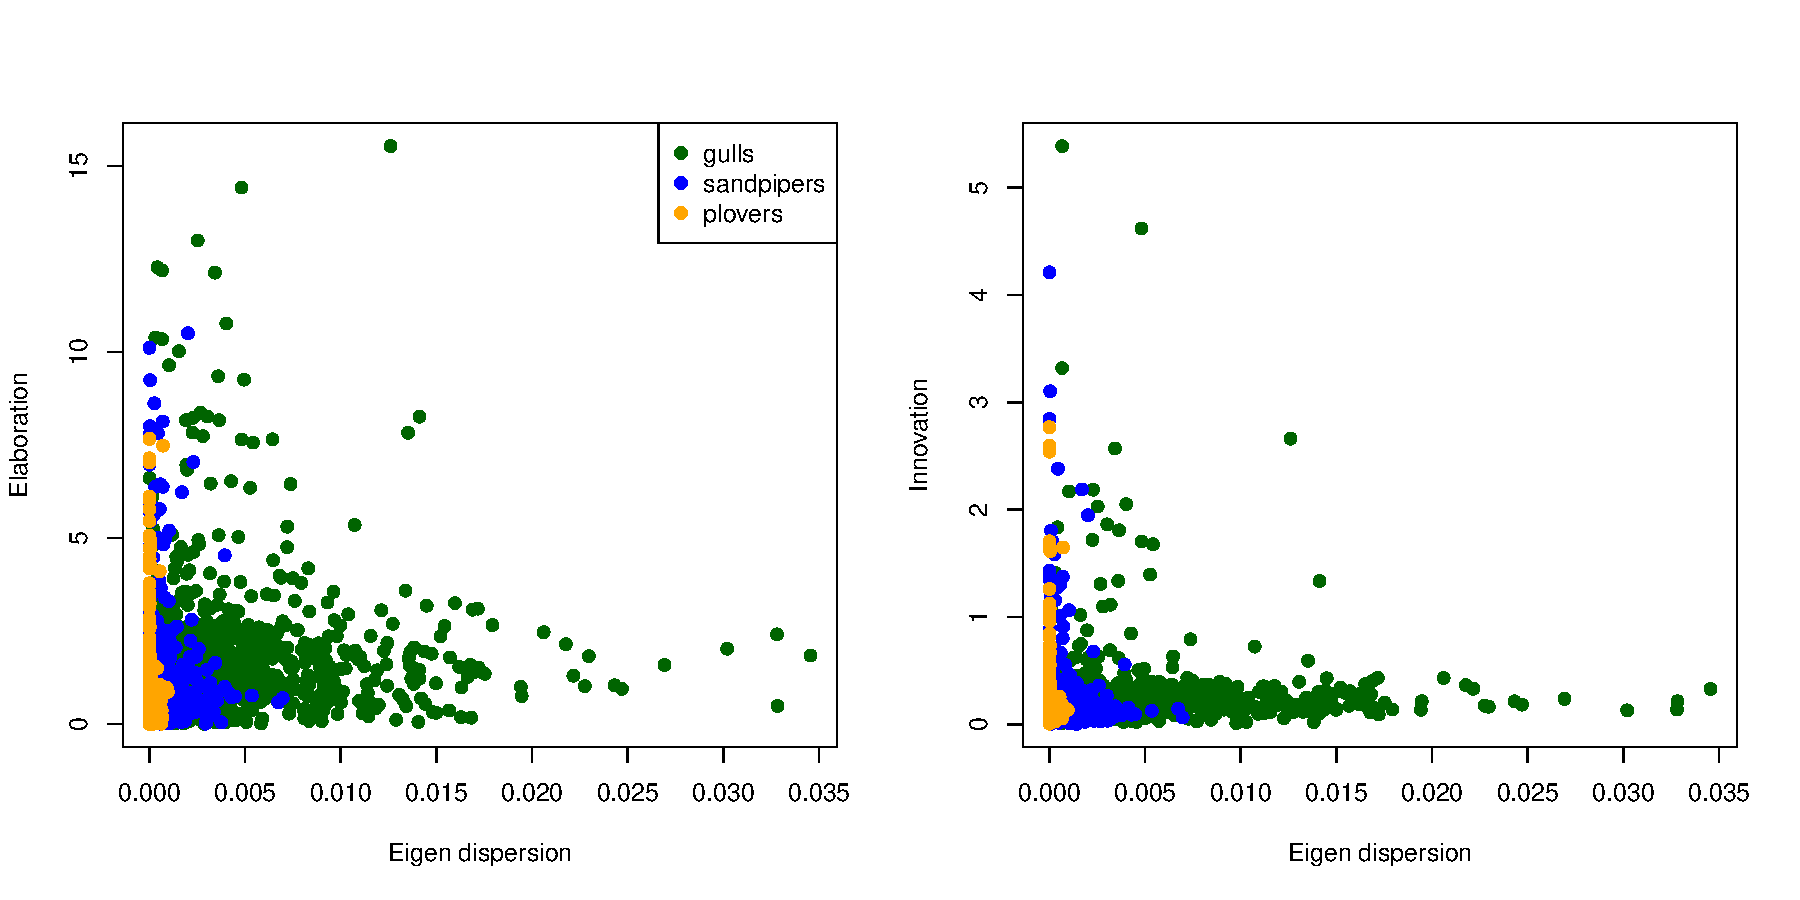
\includegraphics[width=0.9\textwidth]{Figures/elaboration_innovation_dispersion.pdf}
\caption{Relation between relative eigen dispersion [44, 66] %\cite{vanvalen1974,watanabe2022}
and $\text{elaboration}_{\text{clade}_{c}}$ and $\text{innovation}_{\text{clade}_{c}}$ on the \texttt{charadriiformes} example dataset from the \texttt{dispRity} package.}
\label{Fig:eigen_dispersion}
\end{figure}

\subsubsection{Evolvability and respondability}

[42] %\cite{hansen2008measuring}
propose to measure the evolvability and respondability of an individual as their ``response to selection in $n$ traits''.
Here, some equivalent can be drawn (albeit cautiously) between the response of an individual or a group (population) to selection pressure and a species.
Arguably, a species is the end product of this (and many other) selection pressures on a group of individuals.
If so, then, we can relate $\text{evolvability}$ and $\text{respondability}$ [42] %\cite{hansen2008measuring}
for a $species_{x}$ to it's $\text{elaboration}_{\text{species}_{x}}$ and $\text{innovation}_{\text{species}_{x}}$ as follows:

\begin{equation}
\text{evolvability}_{\text{species}_{x}} = \text{elaboration}_{\text{species}_{x}}
\end{equation}

\noindent and, using Pythagorean theorem in a right angled triangle:

\begin{equation}
\text{respondability}_{\text{species}_{x}}  = \sqrt{\text{elaboration}_{\text{species}_{x}}^2 + \text{innovation}_{\text{species}_{x}}^2}
\end{equation}


\begin{figure}[H]
\centering
   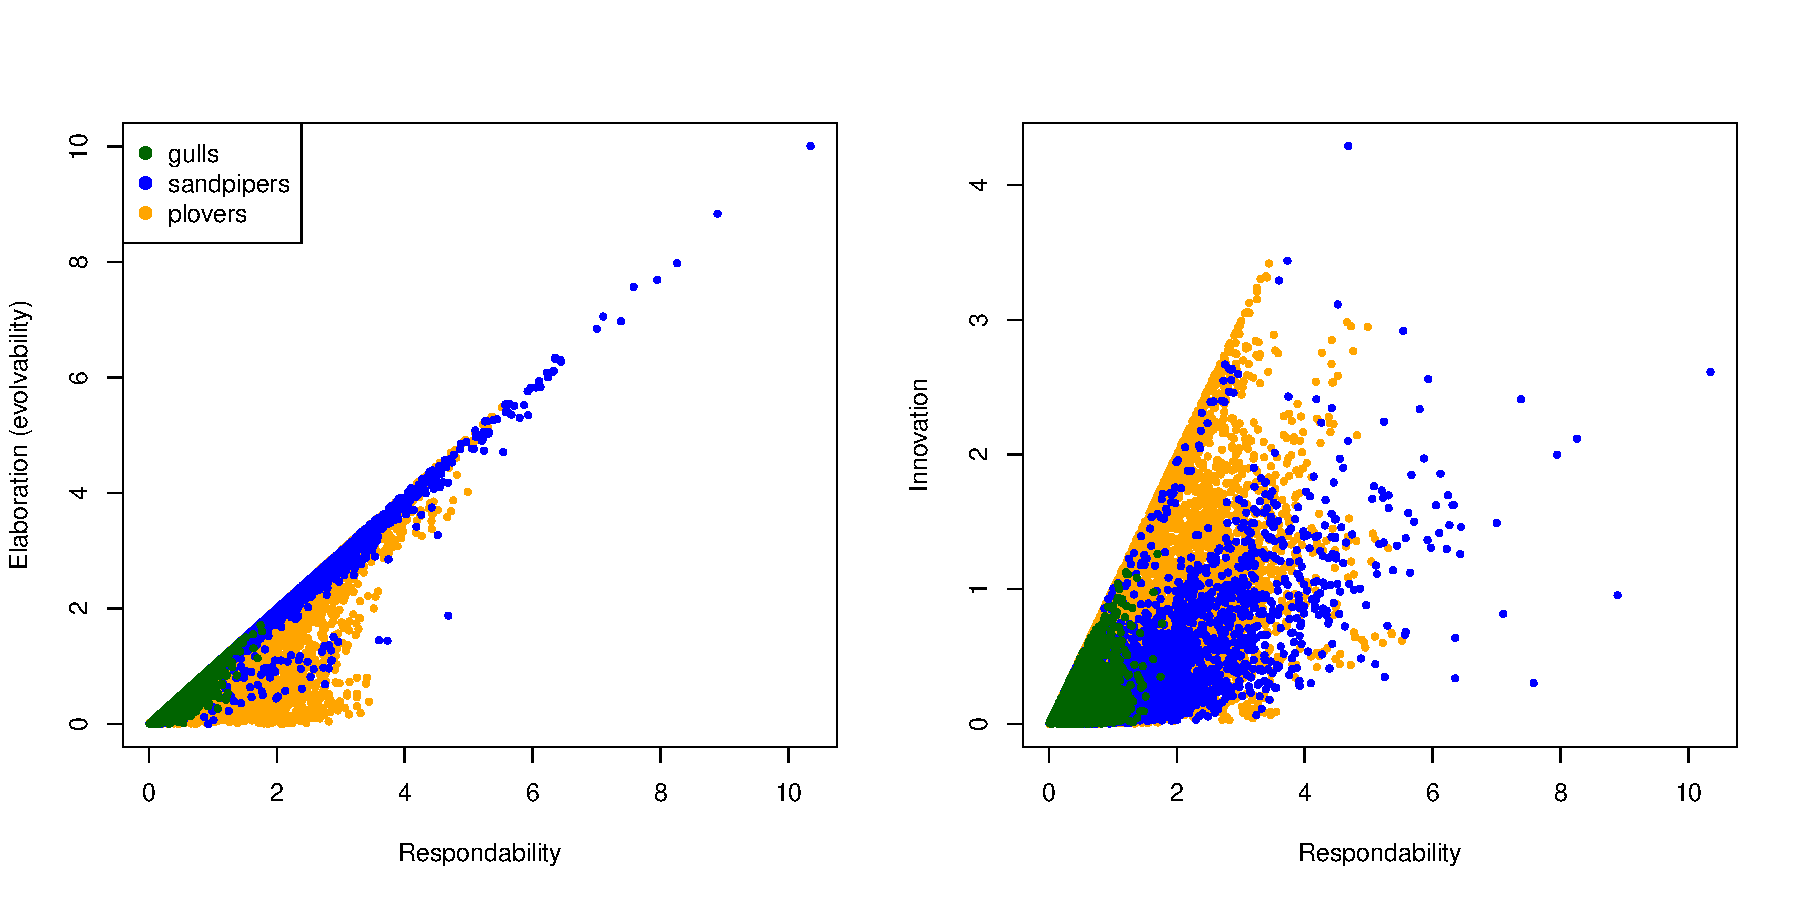
\includegraphics[width=0.9\textwidth]{Figures/respondability.pdf}
\caption{Relation between respondability [42] %\cite{hansen2008measuring}
and $\text{elaboration}_{\text{species}}$ and $\text{innovation}_{\text{species}}$ on the \texttt{charadriiformes} example dataset from the \texttt{dispRity} package.}
\label{Fig:respondability}
\end{figure}

Conditional evolvability however will be more complex to determine since it is defined as the relation between evolvability and autonomy which is specific defined in [42] %\cite{hansen2008measuring}
 as the inverse of the \textbf{G} matrix.
In [42] %\cite{hansen2008measuring}
, the inverse of \textbf{G} is defined as ``the fraction of the genetic variation that is independent of potentially constraining characters'' which in our case will be harder to define.
Although it would technically be possible to use the inverse of the \textbf{R} matrix used here ($VCV_{clade}$), it is unclear what it would represent biologically.

%---------------------------------------------
%
%   references
%
%---------------------------------------------

% \bibliographystyle{naturemag}
% \bibliography{references}

\end{document}